
\documentclass[a4paper,10pt]{article}
\usepackage{graphicx}
%\usepackage[]{./draftwatermark/draftwatermark}
%\SetWatermarkFontSize{100cm}
%\SetWatermarkScale{6}
\newcommand{\HRule}{\rule{\linewidth}{0.5mm}}


%opening
\title{C Event Display (CED) User Manual}
\author{Hauke Hoelbe, DESY}
\date{Mai 2012}

\begin{document}

%\begin{figure}
%\end{figure}

%\maketitle
%\bigskip
%\bigskip
%\bigskip
%\bigskip
%\bigskip
%\bigskip

\begin{titlepage}
\begin{center}
    % Upper part of the page
    
\includegraphics[width=0.15\textwidth]{./desylogo.png}\\[1cm]    
    
    \textsc{\LARGE Deutsches Elektronen-Synchrotron }\\[1.5cm]
    
    \textsc{\Large User Manual}\\[0.5cm]
    
    
    % Title
    \HRule \\[0.4cm]
    { \huge \bfseries C Event Display (CED)}\\[0.4cm]
    
    \HRule \\[1.5cm]
    
    % Author and supervisor
    \begin{minipage}{0.4\textwidth}
    \begin{flushleft} \large
    \emph{Author:}\\
    Hauke  \textsc{H\"olbe}
    \end{flushleft}
    \end{minipage}
    \begin{minipage}{0.4\textwidth}
    \begin{flushright} \large
    \emph{Supervisor:} \\
    Dr. Frank \textsc{Gaede}
    \end{flushright}
    \end{minipage}
    
    %\vspace{1cm}
    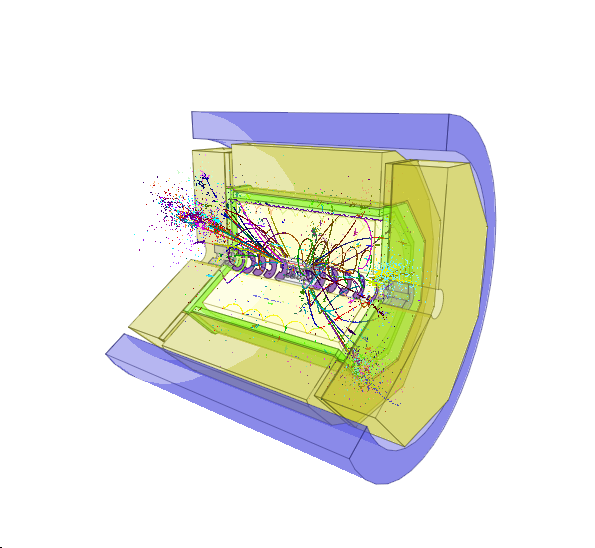
\includegraphics[width=0.8\textwidth]{./title.png}\\[1cm]    
    \vfill
    % Bottom of the page
    %{\large Mai 2012}

    {\large 2011}
    
\end{center}
\end{titlepage}
\newpage

%\begin{abstract}
%test
%\end{abstract}

\tableofcontents
\newpage
\section{Overview}
%\subsection{What CED is}
The C Event Display (CED) and is a client server based tool to draw objects into a dynamic 3D picture. 
CED is a graphical application which uses OpenGL to display the 3D enviroment. 
It is possible to draw individual objects with CED (see section \ref{myviewer}) but for common use it is well integrated into the ilcsoft framework:

The common use for CED is to display events. 
To do this several steps are necessary.
A data file which contains the LCIO objects to be drawn is needed. 
This object gets processed with Marlin, which sends the data of the events over a TCP/IP connection to CED. 
In order to do this, Marlin needs a steering file. 
This XML file can be written by hand or can be generated with MarlinGUI.
The steering file decides which data file is read and also which viewer is used, the viewer decides which datatype is on what layer (see layer section), which color will be used etc. Example viewers are: Generic-, CED- and DST-Viewer.

%\subsection{(0.2 How do you get it)}
\section{Quickstart}
Generating a Marlin steering file can be time consumming, but there is a tool in the CED package which displays the event using a default configuration. 
For a simple first look, source the ini ilcsoft script and use the command: 
\begin{verbatim}
    ced2go <your datafile>
\end{verbatim}
A window which contains the graphical interpretation of your event will open. 
To view the next event press enter in the terminal where you have commited the ced2go command.

All possible options are available from the menu at the top. 
Additional you are able to use shortcuts (see appendix). 
You are also able to change objects by the popup menu by clicking with the right mouse button at one object.

\begin{figure}
    \begin{center}
         \fbox{
         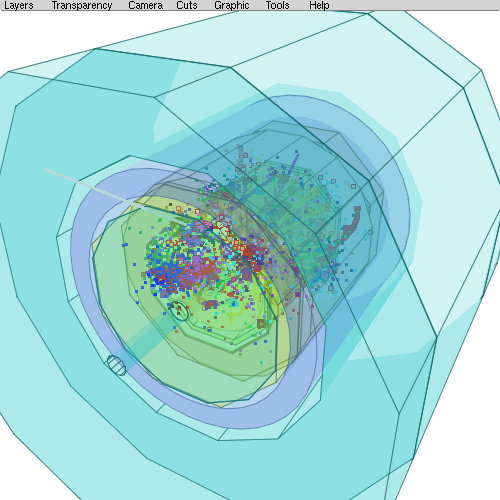
\includegraphics[width=0.5\linewidth]{quickstart1.png}
         }
         \caption{\label{CEDViewer} \textsl{ced2go after the first start}}
    \end{center}
\end{figure}


%\subsection{Help}
%Select the CED window and press 'h' to get an overlay of shortcuts and a description of used layers.

\subsection{menu}
All CED options are accessible from the main menu.
Splitted into seven submenus: 
\begin{itemize}
    \item{Layers}: Toggle the visable of data or detector layers. 
    \item{Transparency}: Change the transparency of the detector components. 
    \item{Camera}: Change the possition of view, reset view or selecting projections. 

    \item{Cuts}: Different cuts of the detector. 

    \item{Graphic}: Graphic options. You can also save your prefered settings here.

    \item{Tools}: Additional functions like making high resolution screenshots.

    \item{Help}: Getting help.

\end{itemize}

\subsection{Pop-up menu}
Right-click on any object displayed in CED open the popup menu. 
This menu allows you to configure or select the selected object.
For example to change the color of the background simply click on it and change a different one.

\section{Save settings}
You are able to save your favorite settings and switch between the saved ones. 
The settings are stored under $\sim$/.glced\_cfg/.
The save function store the current background color, view, transparency, cuts, layers visibility etc. 
But the current event or other Marlin settings is not saved, because these depend on the Marlin steering file and not on CED. 

The config file  is human readable but it is not recommended to change the settings by hand. 

\section{Views}
\subsection{Rotate}
To change the view, simply left-click into the CED window, hold the mouse button and pull in any direction to rotate the view.
\subsection{Zoom factor}
To increase the magnification press '+', to decrease press '-'. If you are on Linux zooming with the mousewheel works too. 
%%here

\subsection{Move}
To move the center of view to any direction, press and hold the middle mouse button and pull. 
\newline\newline
To move the detector on the z-axis, press arrow key $\uparrow$ or $\downarrow$. 

\subsection{Center}
It is possible to center any data object drawn within CED. Simply put your mouse cursor over that object and press 'c' 

\subsection{Side view}
To view the detector from the side press 's', or choose it from the pop-up menu under 'View $\rightarrow$ Side view'.

\subsection{Front view}
To view the detector from front press 'f', or choose it from the pop up-menu under 'View $\rightarrow$ Front view'.

\subsection{Reset view settings}
To reset the view and cut settings press 'r', or choose it from the pop up menu under 'View $\rightarrow$ Reset view'. This option resets: perspective, cutting, projections and zoom level.

\section{Projections}
There is a big difference between views and projections: View options show the same objects at a different angle, in contrast to projections which change the objects. 

\subsection{Side view projection}
To enable side view projection press capital 'S', or choose it from the pop-up menu under 'View $\rightarrow$ Toggle side view projection'. This projection turns the view into side view, and transforms all data (hits, tracks, etc) so that the distance from the beamline to the object are the same as in 3D mode.
\newline\newline
$y_{proj} = \pm \sqrt{x^2 + y^2}$\newline
$x_{proj}=0$\newline
$z_{proj} = y$ \newline
\newline
The detector is cut at $\phi=0$ to enable a view into it. The ability to rotate will be disabled. To exit this projection and get back to the previous view choose the side view projection mode again, or press 'S'. 




\subsection{Front view projection}
To enable front view projection press capital 'F', or choose it from the pop-up menu under 'View $\rightarrow$ Toggle front view projection'. This projection turns the view into front view, and transforms all data (hits, tracks etc)
($z_{proj} = 0$). The perspective is turned off and the detector is cut at z=0 to enable a view into the detector. The ability to rotate is disabled. To exit this projection, press 'F' or choose the front view projection mode again. 

\begin{figure}[h!]
\begin{minipage}[t]{6cm}
\centerline{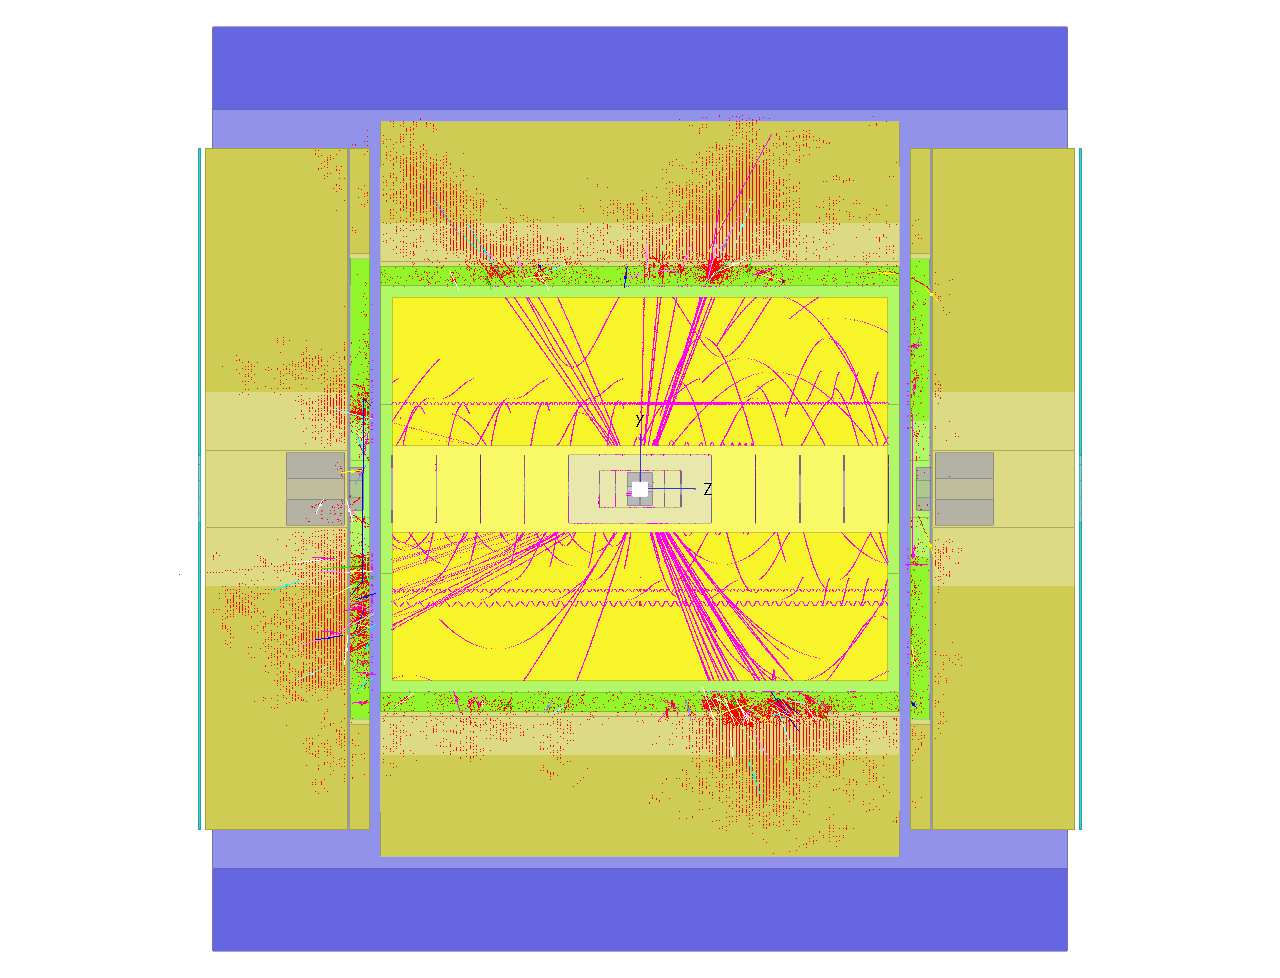
\includegraphics[height=5cm]{sideview2.png}}
\caption{\label{CEDViewer} \textsl{Side view projection}}
\end{minipage}
\hfill
\begin{minipage}[t]{6cm}
\setlength{\fboxsep}{0mm}
\centerline{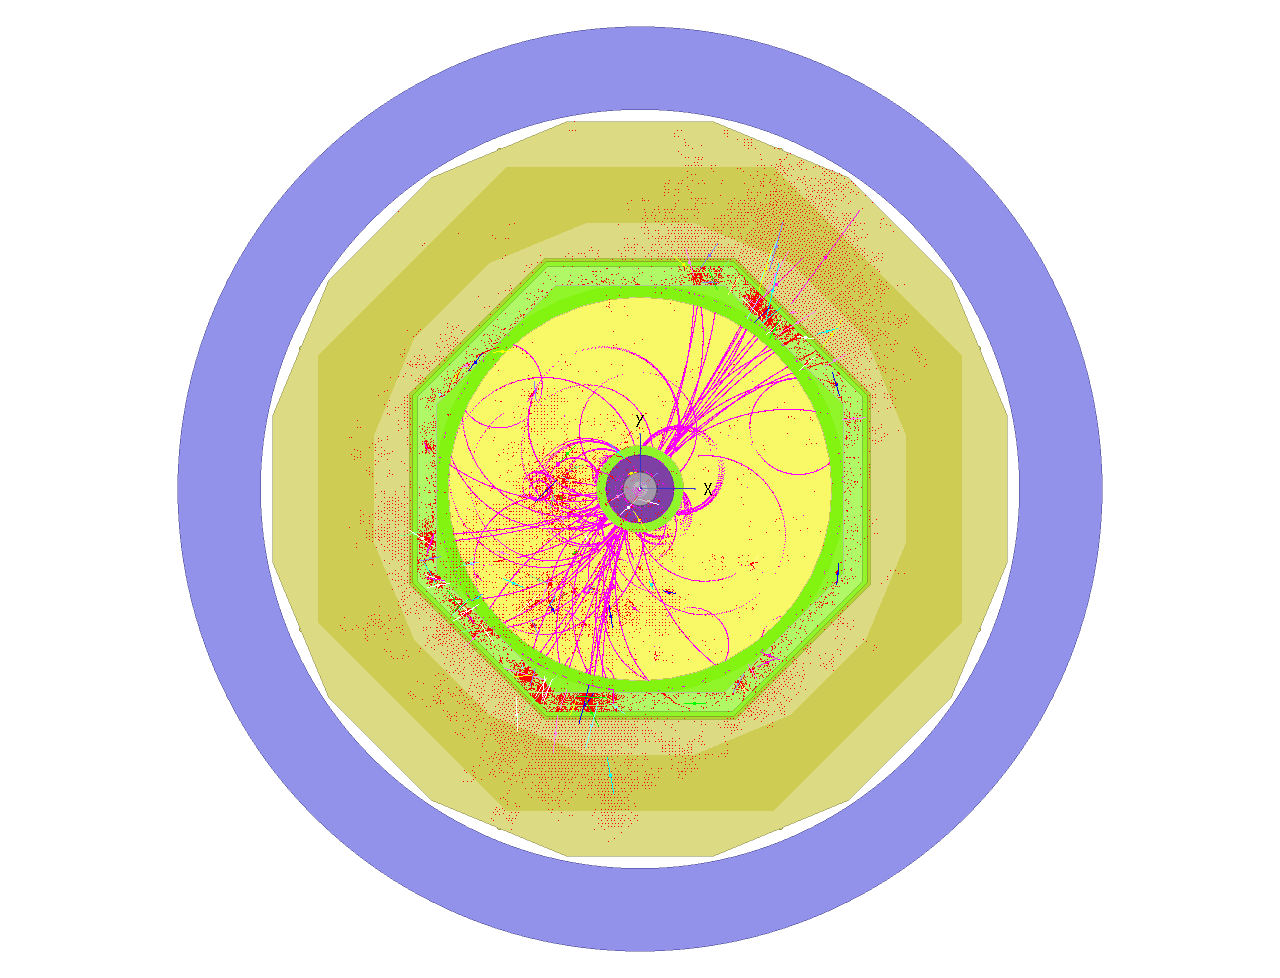
\includegraphics[height=5cm]{frontview2.png}}
\caption{\label{DSTViewer}\textsl{Front view projection}}
\end{minipage}
\end{figure}

\subsection{Fisheye view}
This projection enlarges the inner region of the detector, to give a clearer view to the inner tracks and hits of the event. To enable fisheye press 'v' or select it from the pop-up menu under 'View $\rightarrow$ Toggle fisheye projection'. To turn this projection off, press 'v', or select it from the pop-up menu again. The fisheye projection is usable together with the front or side view projection.

\begin{figure}[h]
\centerline{ 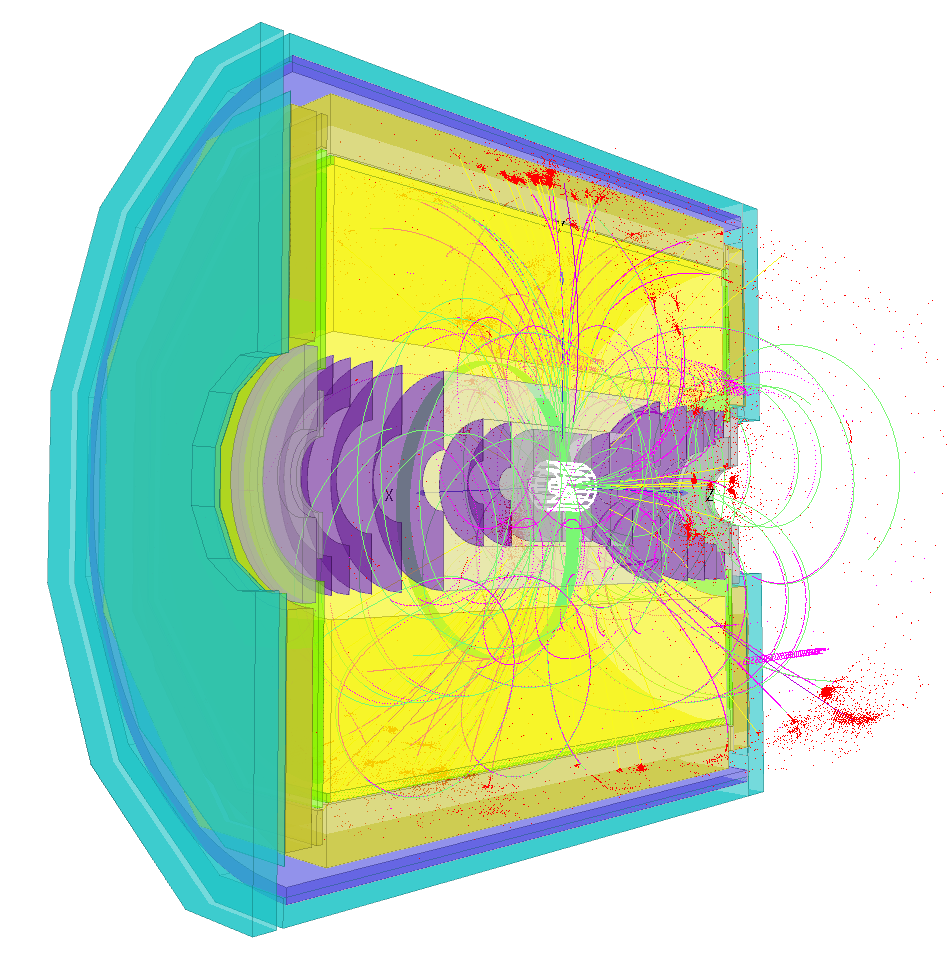
\includegraphics[height=6cm]{fisheye1.png}}
\caption{\label{CEDViewer} \textsl{Fisheye projection}}
\end{figure}

\section{Layer}
With CED it is possible to draw different data on different layers. This allows to show or hide specific types of data while working with CED. Both data and detector components are placed on layers. CED supports 100 different layers, but you are only able to toggle the visibility of the first 25 data layers and the first 20 detector layers at runtime. 

\subsection{Data Layer}
To show which data is actually on which layer, open the overlaying help by pressing 'h', or choose 'Data layers' from the pop-up menu. To toggle the visibility of data layers quickly, there are shortcuts for the first 25 data layers. See section 'Shortcuts'. 
\newline\newline
It is possible to turn all data layers simultaneously on or off by selecting 'Data layers $\rightarrow$ Show/Hide all data layers', or by pressing '$`$'

\subsection{Detector components}
Also detector components can lie on layers. To toggle the visibility of detector components choose the corresponding component from 'Detector layers' in the pop up menu. It is possible to turn all components simultaneously on/off by selecting 'Detector components $\rightarrow$ Show/Hide all detector components'. 

\begin{figure}[h]
\centerline{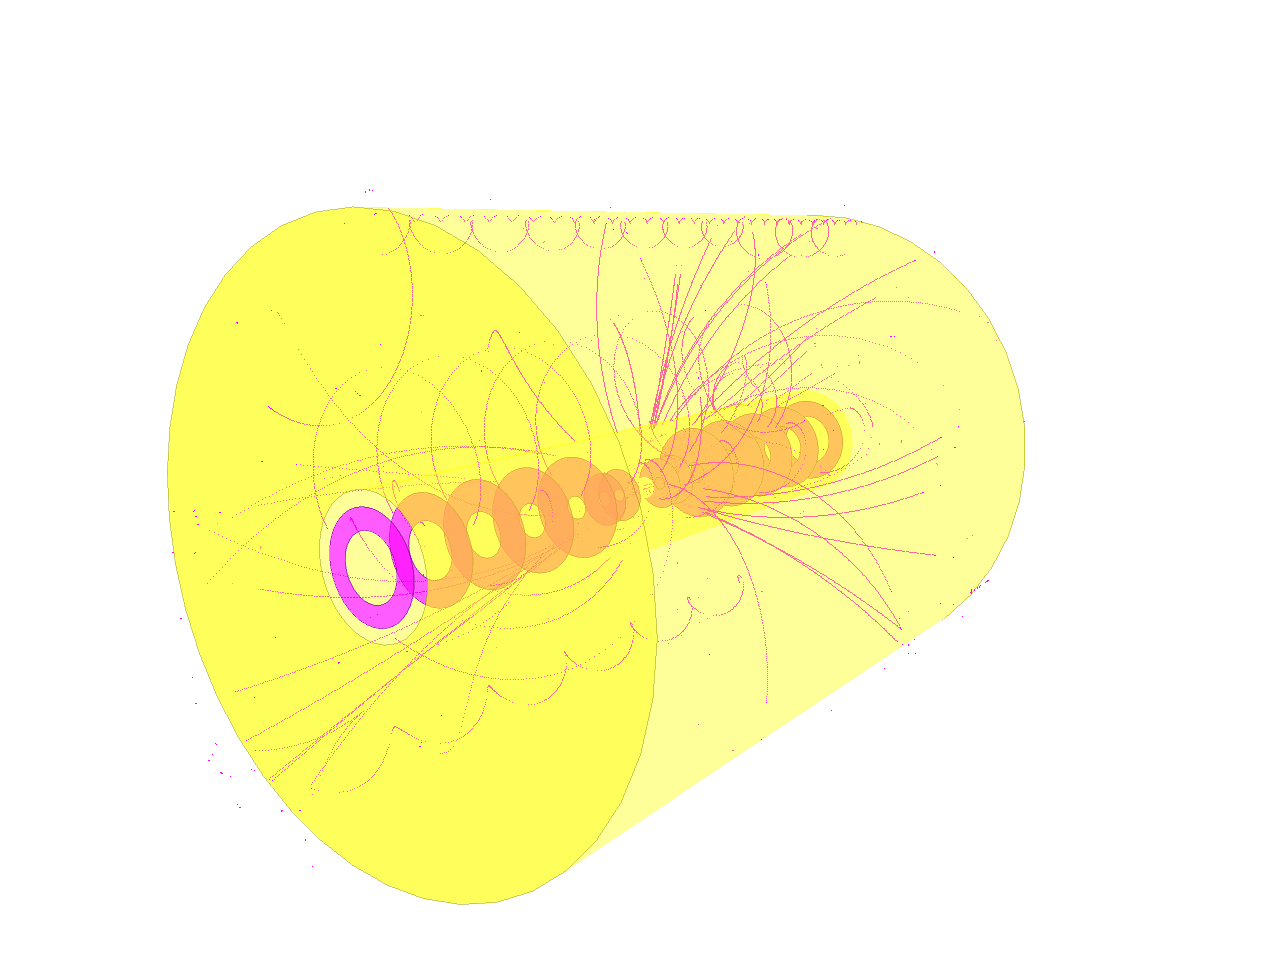
\includegraphics[height=6cm]{detector_layer.png}}
\caption{\label{detectorlayer} \textsl{Detector components: Some detector layers are turned off}}
\end{figure}

\section{Cuts}
In CED it is possible to cut a given range of phi out of the detector, or cut data and detector at a specific z-axes value.

\subsection{Longitudinal cuts}
To cut down the detector in length, press and hold capital 'Z', to enlarge the detector back, press and hold 'z'.

\subsection{Phi cuts}
To cut off a pie slice from the detector, select 'Detector cuts $\rightarrow$ Angle' from the pop-up menu. Available angles are: 0, 30, 90, 135, 180, 270 and 360 degrees. 


\begin{figure}[h]
\begin{minipage}[t]{6cm}
\centerline{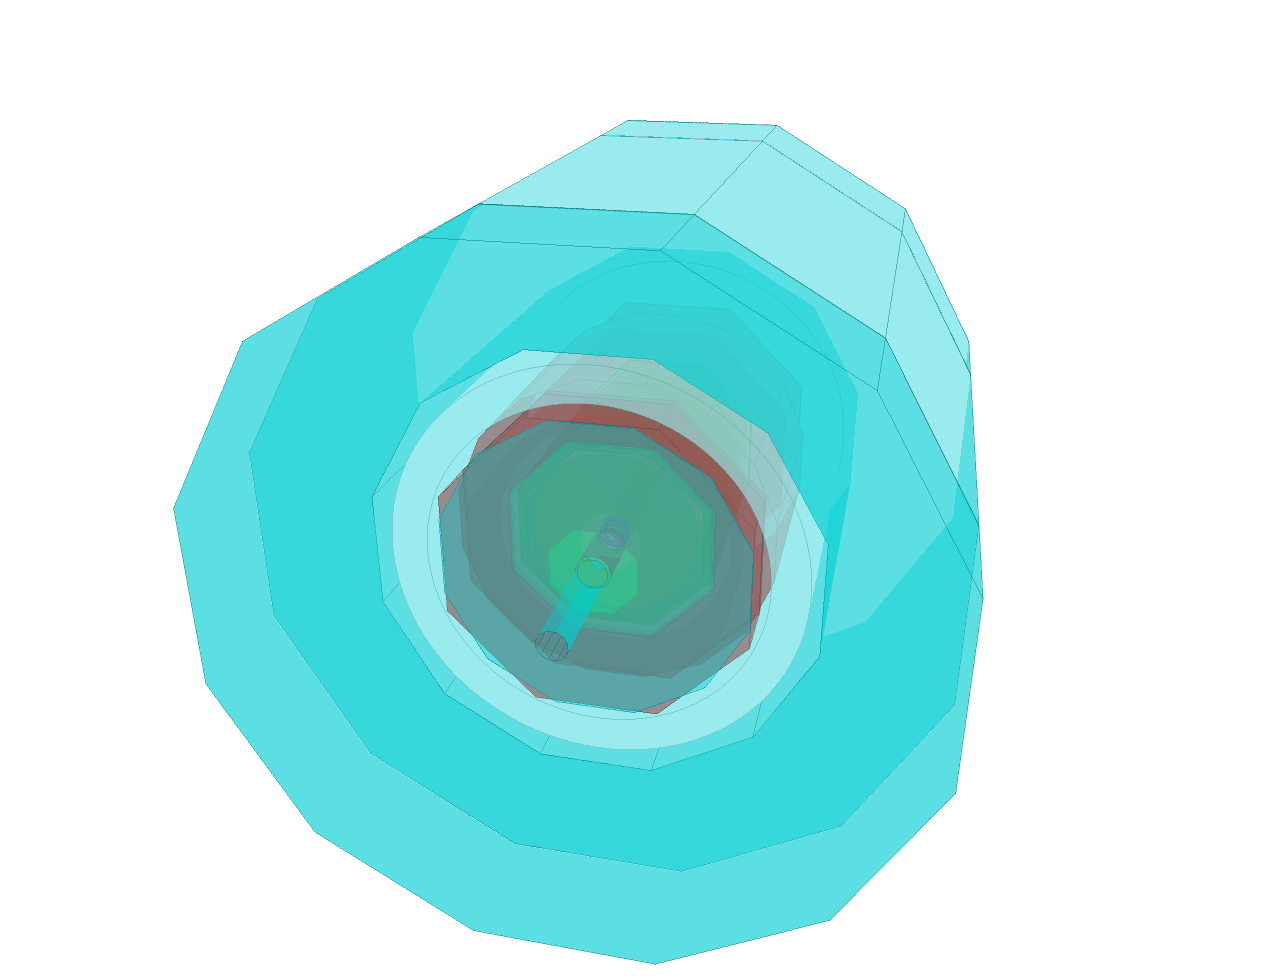
\includegraphics[height=6cm]{phi_cut_0.png}}
\caption{\label{CEDViewer} \textsl{Phi cut 0}}
\end{minipage}
\begin{minipage}[t]{6cm}
\setlength{\fboxsep}{0mm}
\centerline{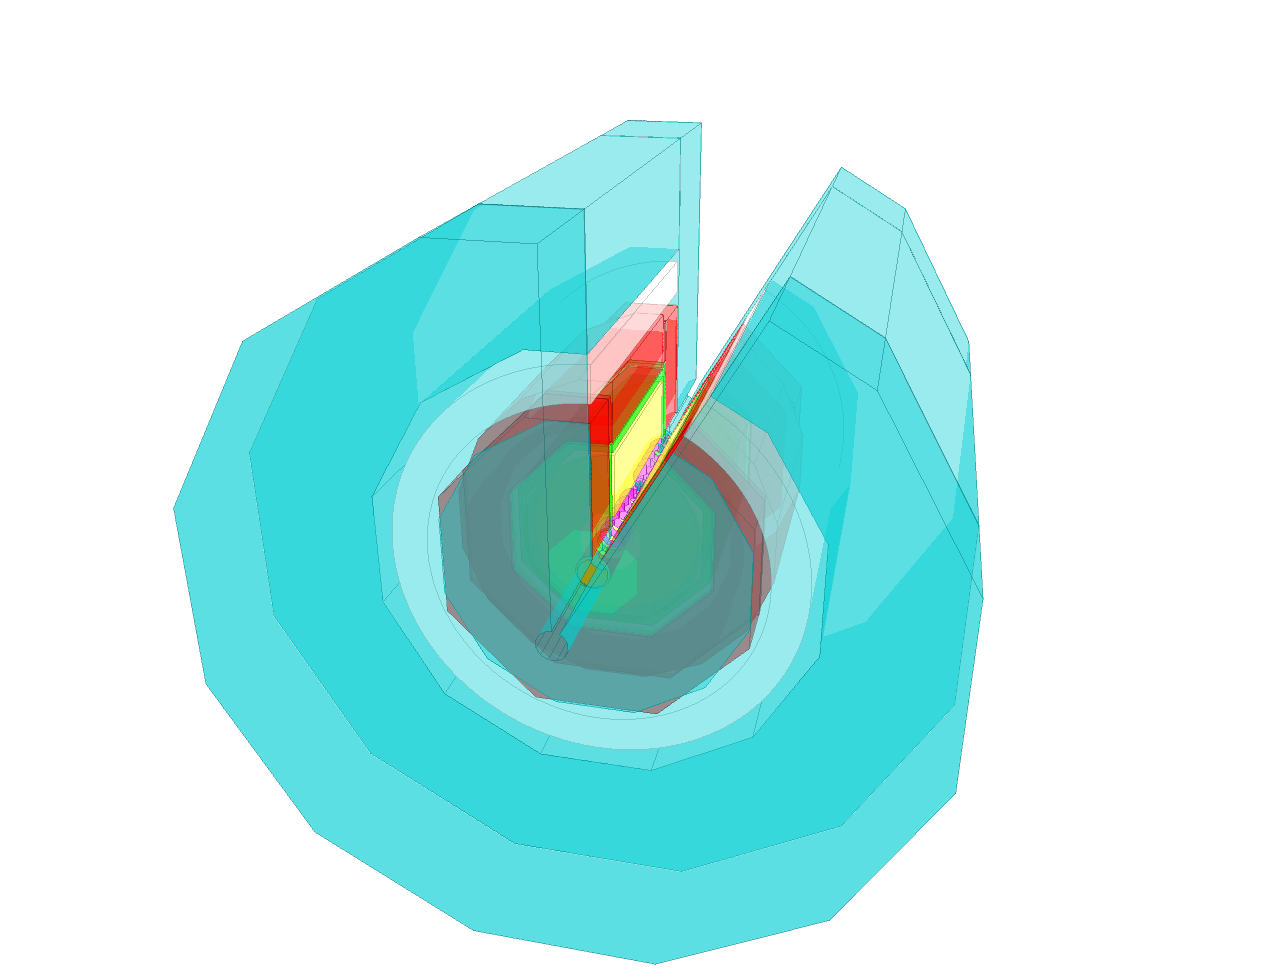
\includegraphics[height=6cm]{phi_cut_30.png}}
\caption{\label{DSTViewer}\textsl{Phi cut 30}}
\end{minipage}

\end{figure}
\begin{figure}[h]
\begin{minipage}[t]{6cm}
\centerline{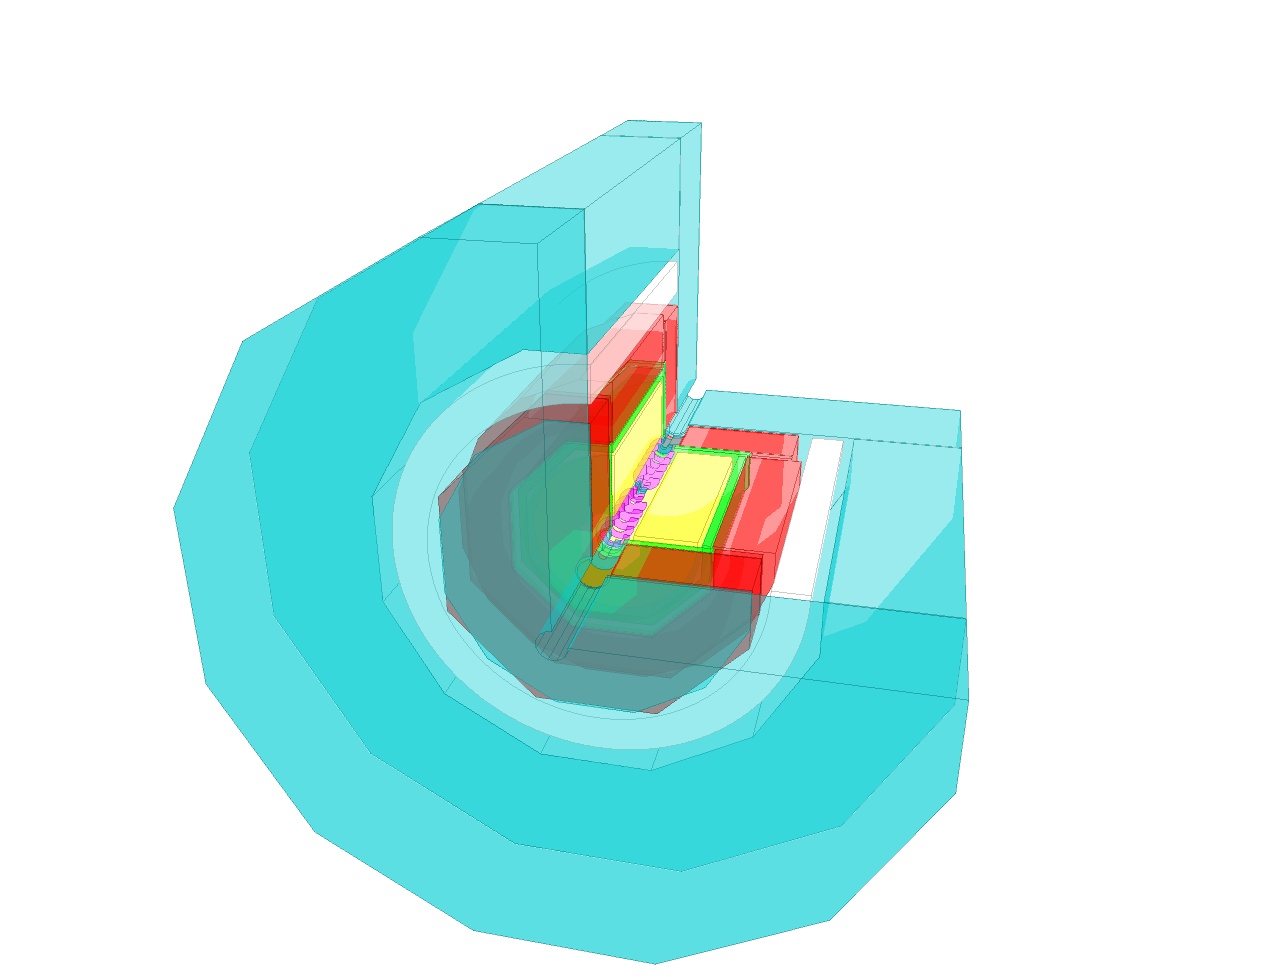
\includegraphics[height=6cm]{phi_cut_90.png}}
\caption{\label{CEDViewer} \textsl{Phi cut 90}}
\end{minipage}
\begin{minipage}[t]{6cm}
\setlength{\fboxsep}{0mm}
\centerline{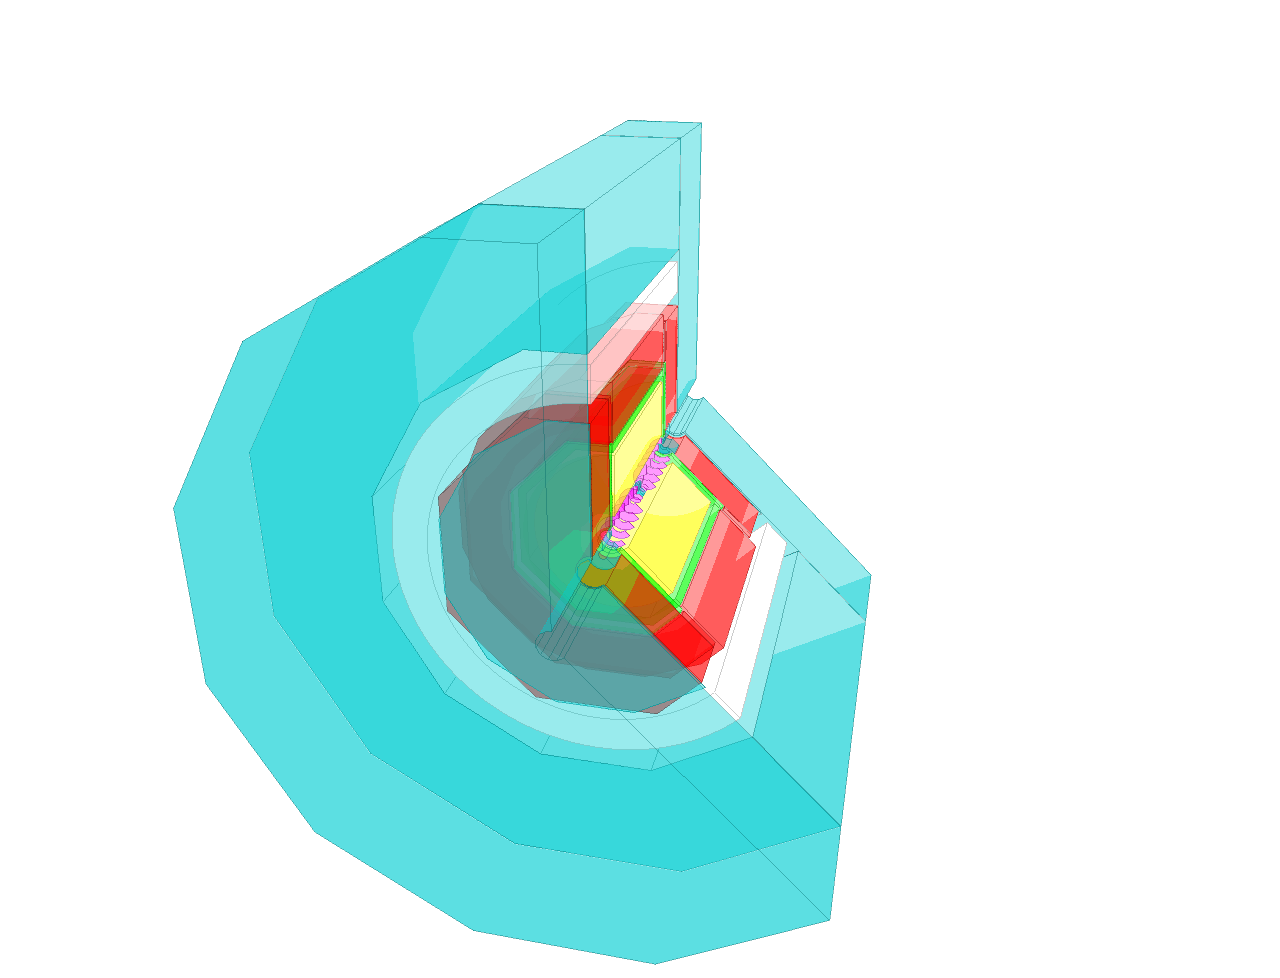
\includegraphics[height=6cm]{phi_cut_135.png}}
\caption{\label{User viewer}\textsl{Phi cut 135}}
\end{minipage}

%\end{figure}
%\begin{figure}[h]
%\setlength{\fboxsep}{0mm}
%\centerline{\fbox{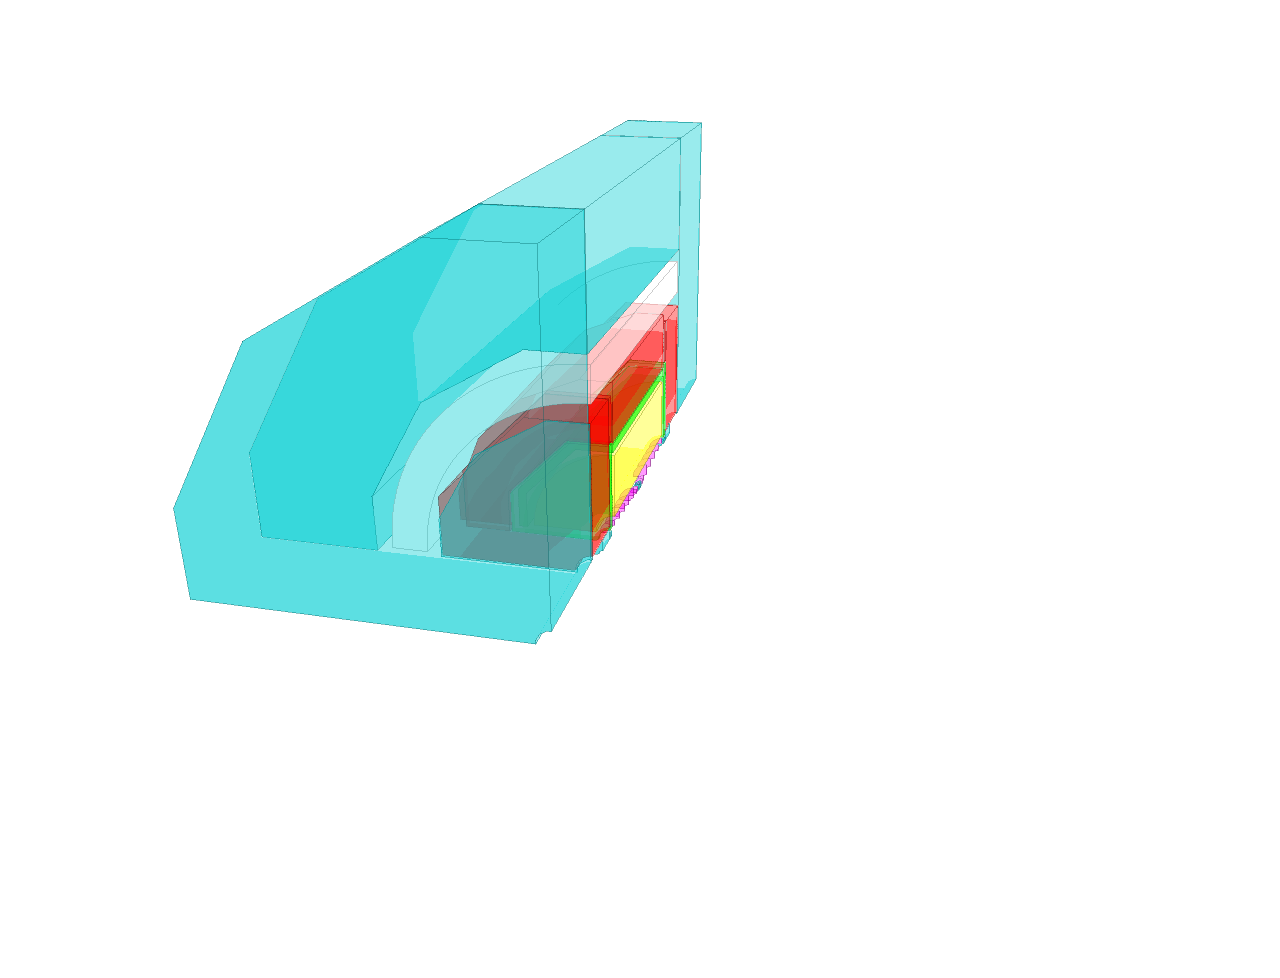
\includegraphics[height=6cm]{phi_cut_270.png}}}
%\caption{\label{User viewer}\textsl{Phi cut 270}}
\end{figure}


\section{Background color}
Changing the background color is not only a setting to increase the aesthetic of the picture, it can also be used to increase the visiblility of the drawn data.
\subsection{Change background color}
To toggle the background color choose a color from the pop-up menu under 'Background color', or press 'b' to change the color from blue to black, over gray to white.

\begin{figure}[h]
\begin{minipage}[t]{6cm}
\centerline{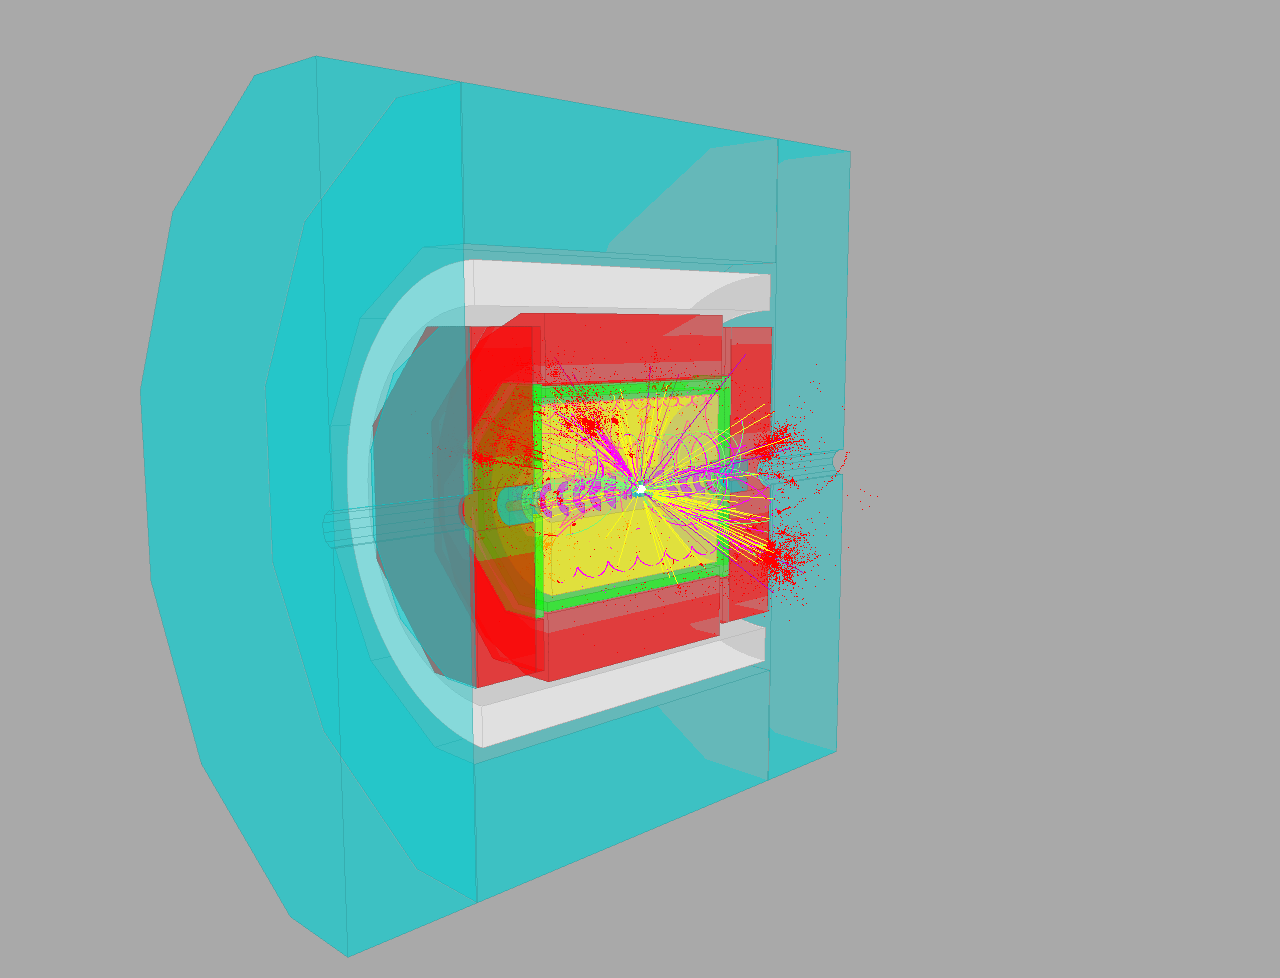
\includegraphics[height=4.5cm]{bg_color_dackgray1.png}}
\caption{\label{CEDViewer} \textsl{Background color: darkgray}}
\end{minipage}
\hfill
\begin{minipage}[t]{6cm}
\setlength{\fboxsep}{0mm}
\centerline{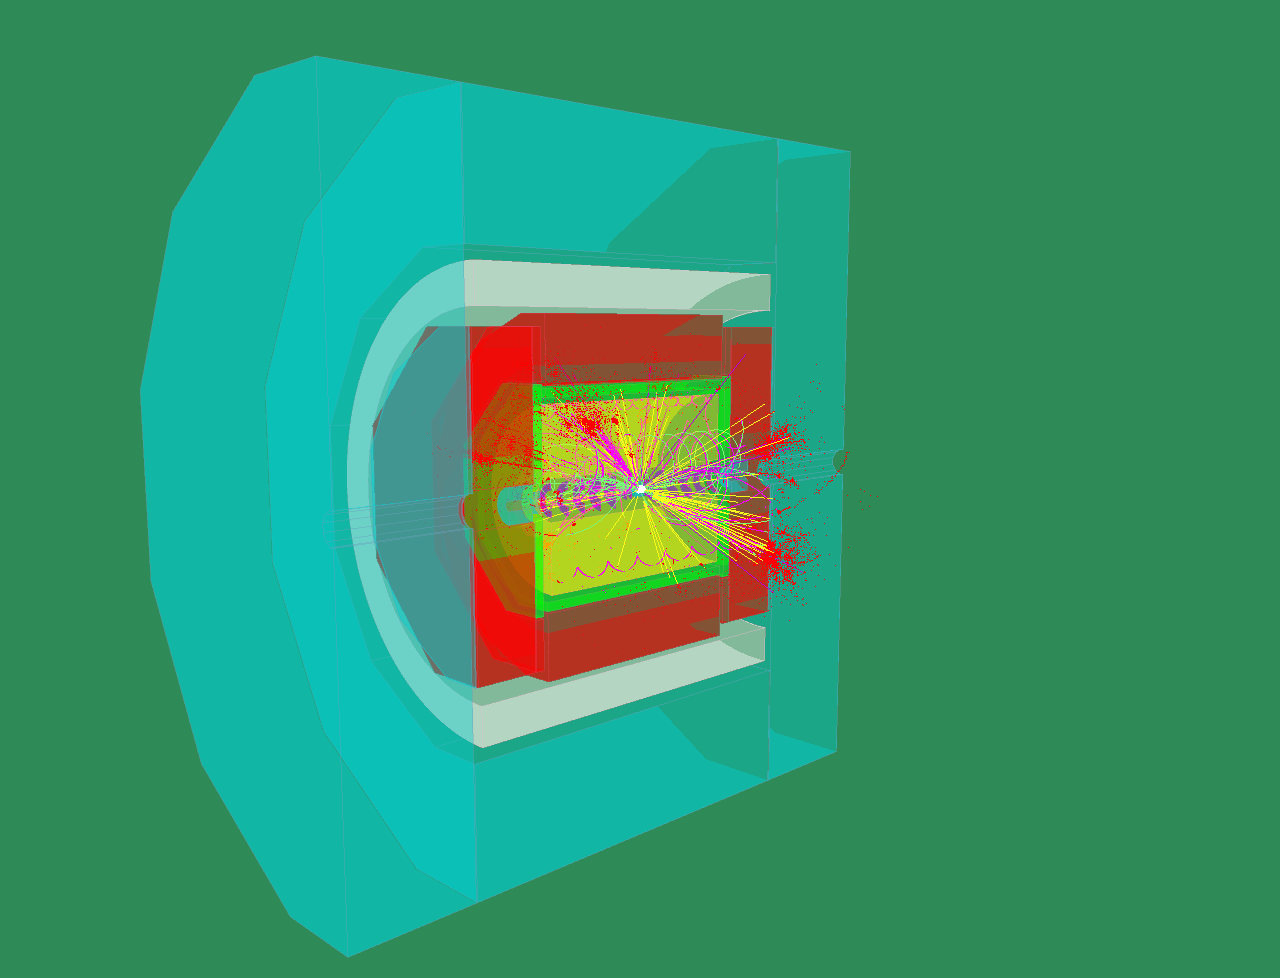
\includegraphics[height=4.5cm]{bg_color_green1.png}}
\caption{\label{DSTViewer}\textsl{Background color: green}}
\end{minipage}
\end{figure}

\begin{figure}[h]
\begin{minipage}[t]{6cm}
\centerline{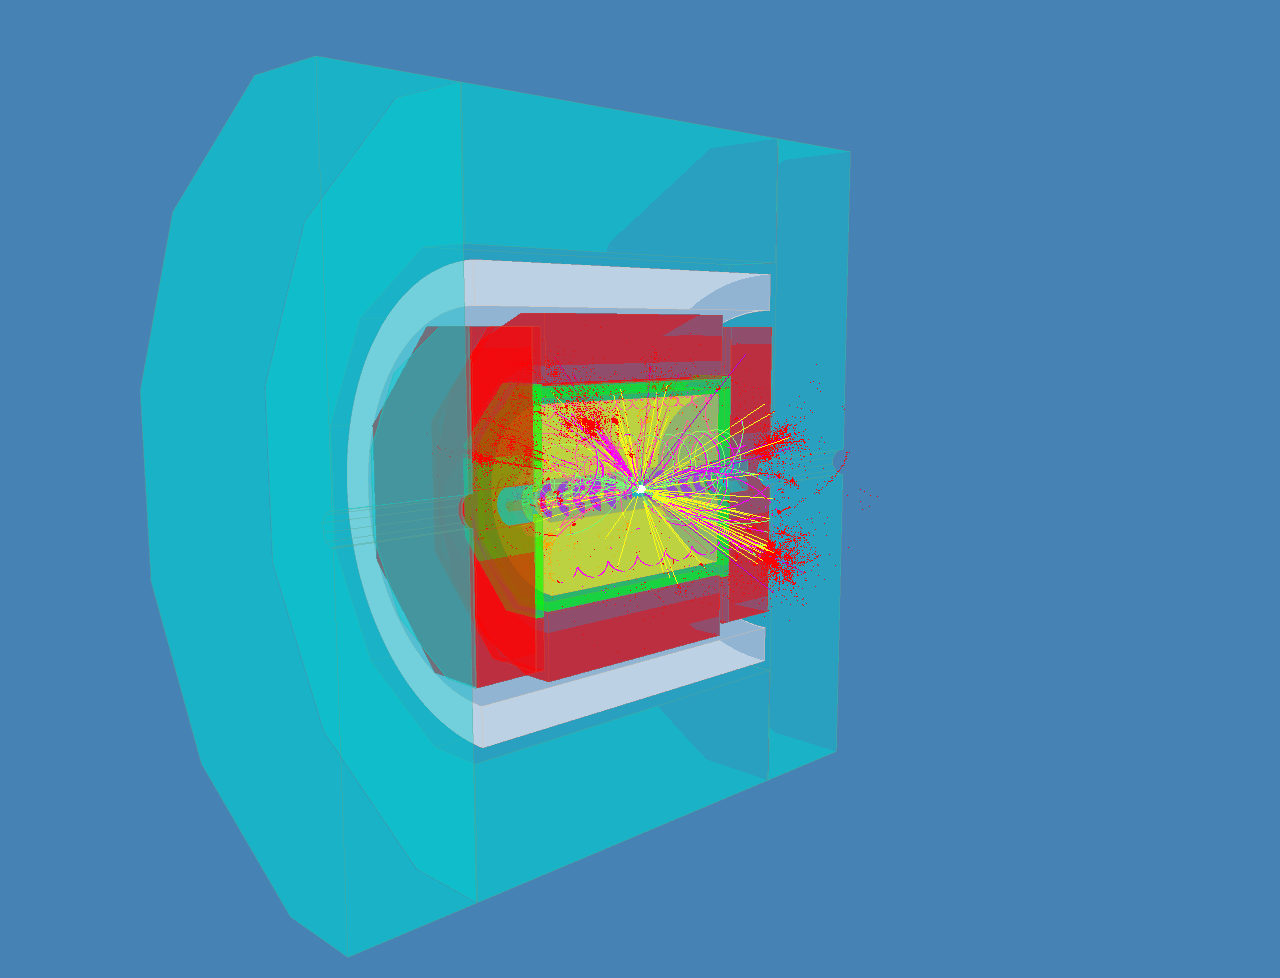
\includegraphics[height=4.5cm]{bg_color_blue1.png}}
\caption{\label{CEDViewer} \textsl{Background color: blue}}
\end{minipage}
\hfill
\begin{minipage}[t]{6cm}
\setlength{\fboxsep}{0mm}
\centerline{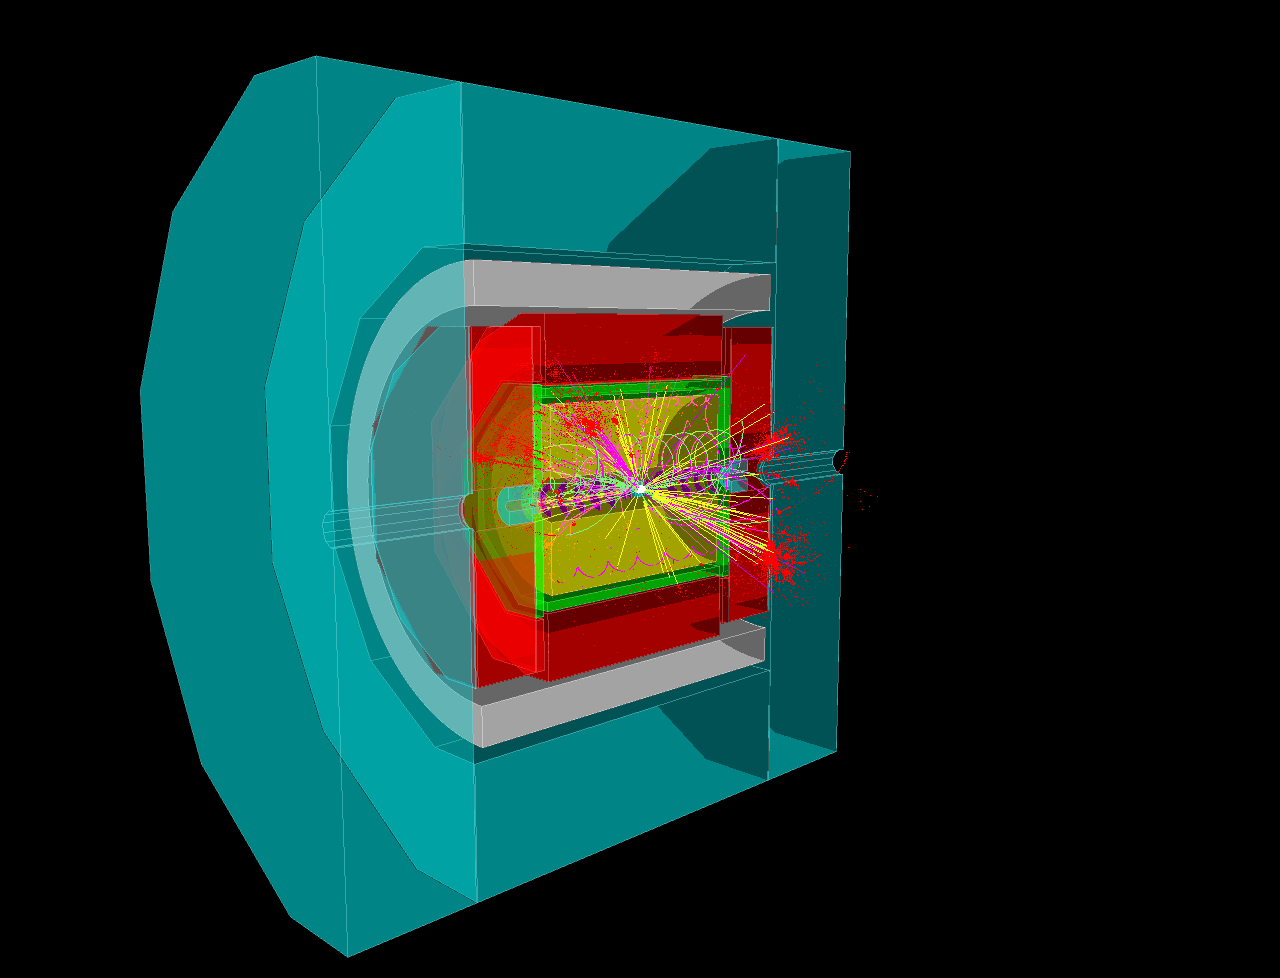
\includegraphics[height=4.5cm]{bg_color_black1.png}}
\caption{\label{User viewer}\textsl{Background color: black}}
\end{minipage}
\end{figure}

\begin{verbatim}
	glced -bgcolor 0xXXXXXX
\end{verbatim}

X stands for a number from 0 till F.
For some examples see Figure \ref{html}
\begin{figure}[h]
\setlength{\fboxsep}{0mm}
\centerline{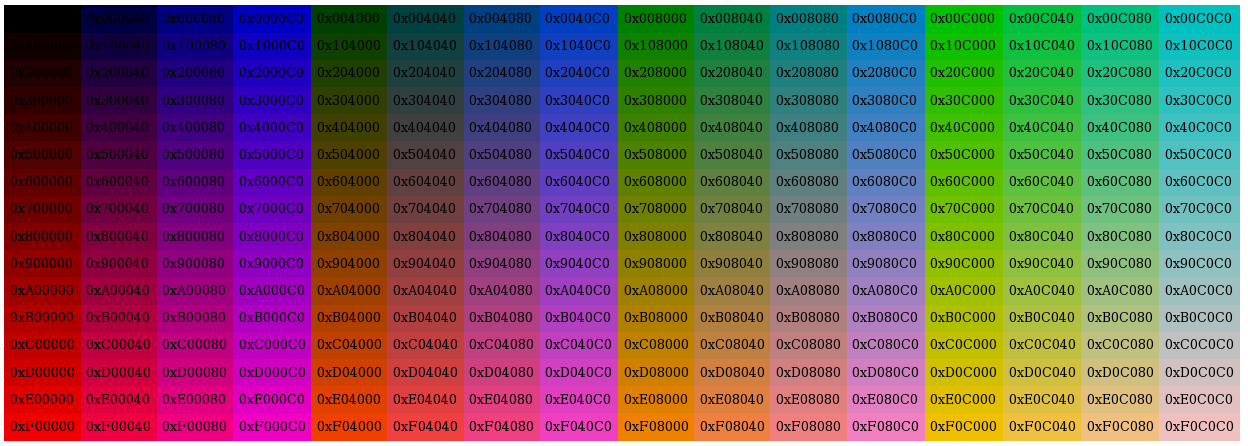
\includegraphics[width=1\linewidth]{html_colors1.png}}
\caption{\label{html}\textsl{Some HTML color codes}}
\end{figure}

\section{Graphical options}
There are a lot of options to customize the look of CED.

\subsection{Differences between classic and new view}
To toggle between classic and new view chose 'Graphics options $\rightarrow$ Classic view' or 'Graphics options $\rightarrow$ New view' from the pop up menu. There are two graphical settings which are affected by this option:
 \begin{center}
 \begin{tabular}[ht]{|l|c|c|}
  \hline
  &Classic view & New view\\
  \hline
  Detector look & mesh & transparency\\
  perspective & flat & 3D\\
  \hline
\end{tabular}
\end{center}

\begin{figure}[h]
\begin{minipage}[t]{6cm}
\setlength{\fboxsep}{0mm}
\centerline{\fbox{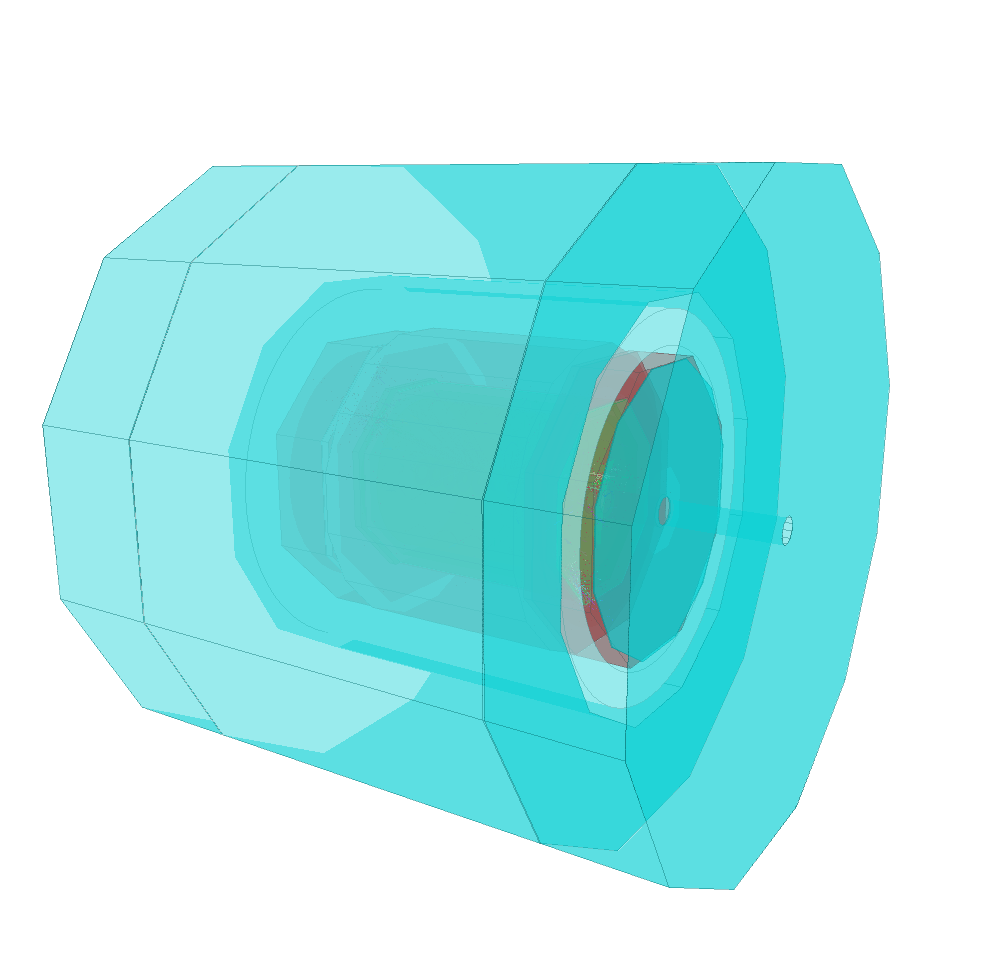
\includegraphics[height=5.5cm]{new_view1.png}}}
\caption{\label{CEDViewer} \textsl{New view}}
\end{minipage}
\hfill
\begin{minipage}[t]{6cm}
\setlength{\fboxsep}{0mm}
\centerline{\fbox{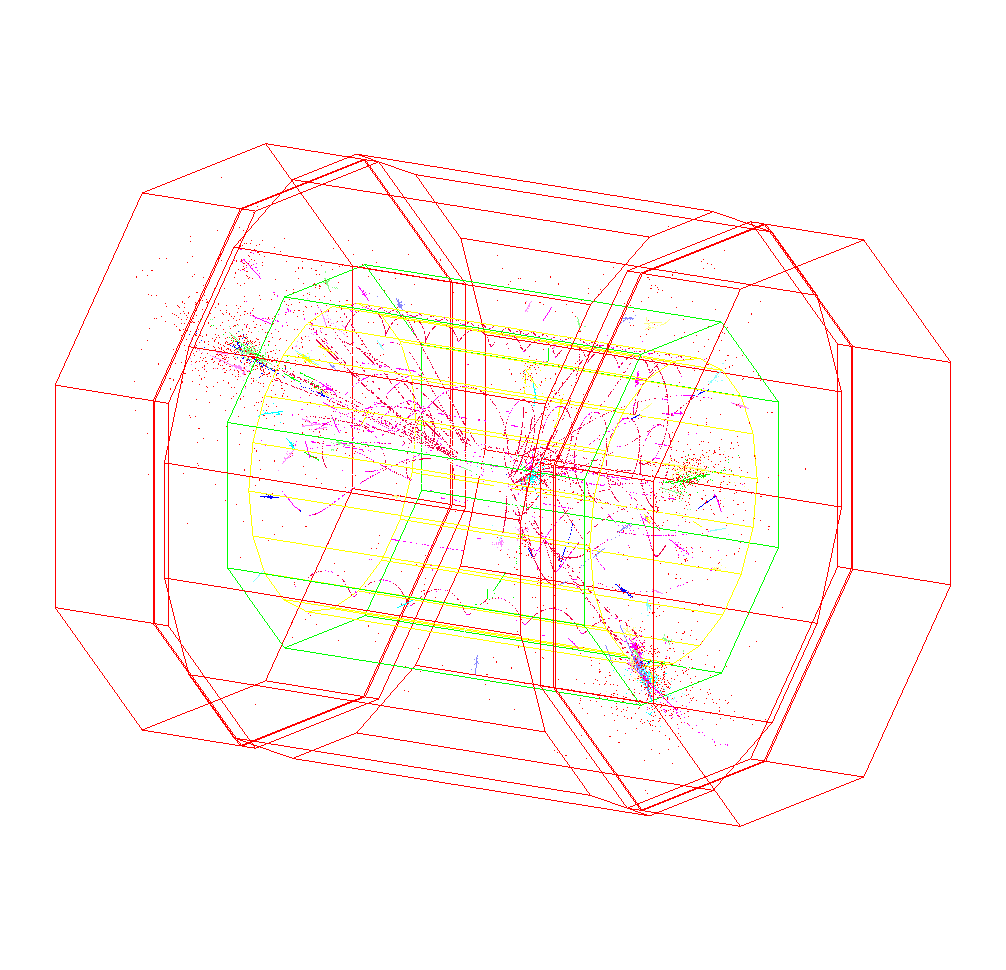
\includegraphics[height=5.5cm]{classic_view1.png}}}
\caption{\label{DSTViewer}\textsl{Classic view}}
\end{minipage}
\end{figure}


\subsection{Perspective setting}
To turn the perspective on or off, select 'Graphics options $\rightarrow$ Graphic details $\rightarrow$ Perspective' from pop-up menu. Perspective on means, that objects which are further away from the viewer appear smaller. Perspective off means, all objects have the same size, however far away they are. 

\subsection{Transparency or mesh view}
To change the way the detector is drawn, select 'Graphics options $\rightarrow$ Graphic details $\rightarrow$ Transparency/mesh' from pop up-menu.
\subsection{Visibility of coordinate axes}
Per default at x=0, y=0, z=0 three arrows are drawn standing for the three axes, to turn this off select 'Graphics options $\rightarrow$ Graphic details $\rightarrow$ Toggle visible of axes' from pop-up menu

%\begin{center}
%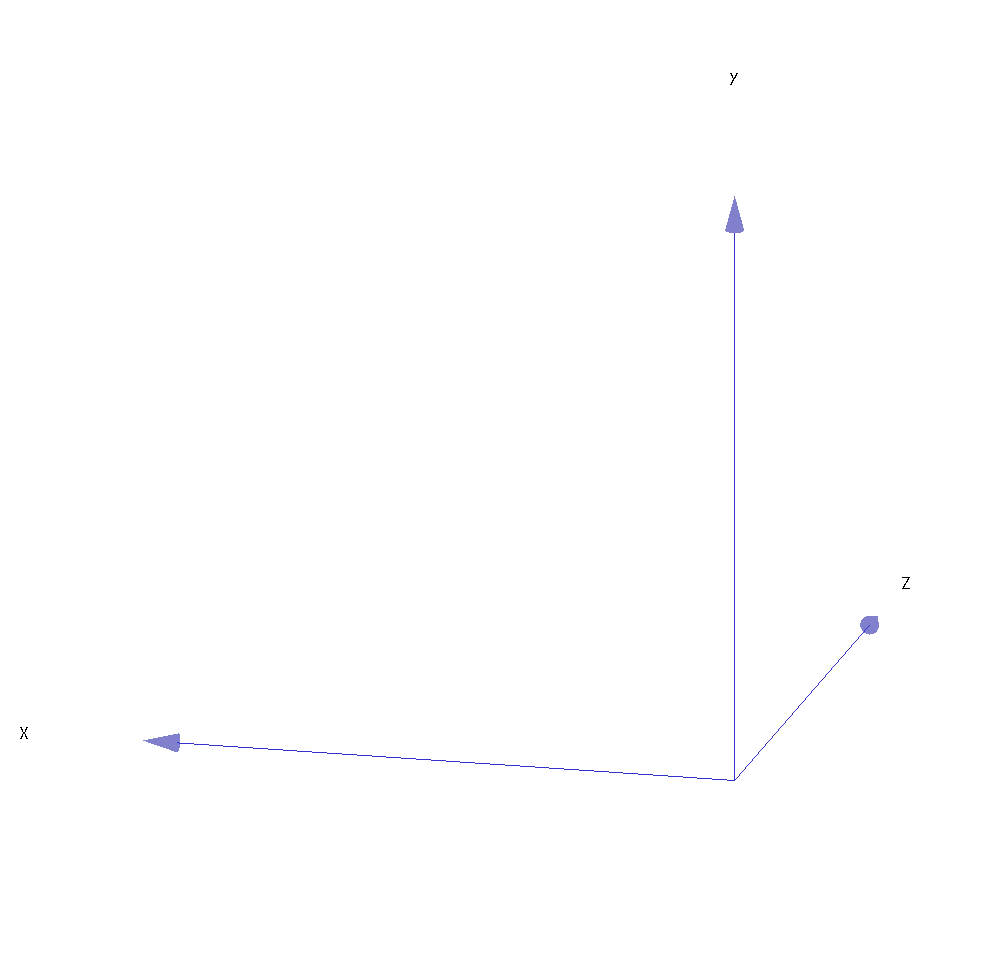
\includegraphics[width=4cm]{axes1.png}
%\end{center}

\subsection{Transparency value}
While not in mesh view, it is possible to change the value of detector transparency by selecting 'Graphics options $\rightarrow$ Transparency value $\rightarrow$ percent of transparency' from pop-up menu. Possible values are: 0, 40, 60, 70, 80, 90, 95 and 100\%.


\begin{figure}[h!]
\begin{minipage}[t]{6cm}
\setlength{\fboxsep}{0mm}
\centerline{\fbox{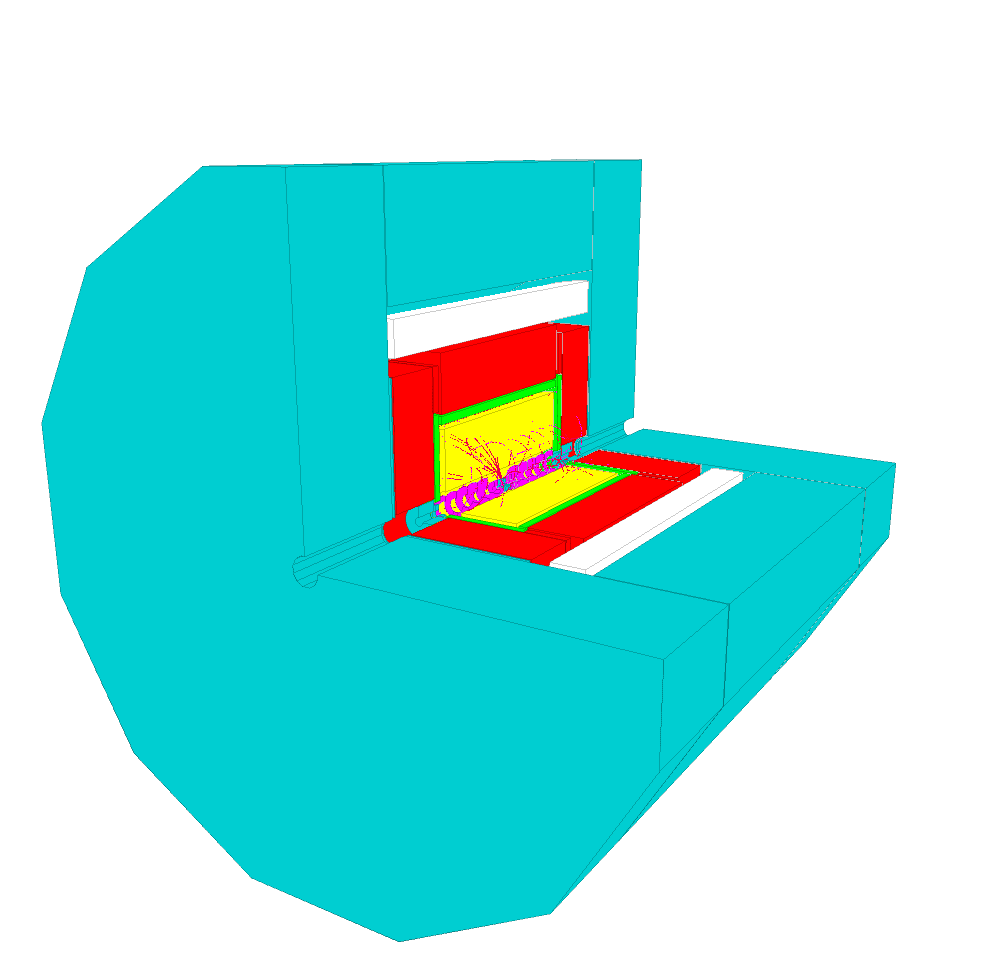
\includegraphics[height=5.5cm]{transparency_0.png}}}
\caption{\label{CEDViewer} \textsl{Transparency 0\%}}
\end{minipage}
\hfill
\begin{minipage}[t]{6cm}
\setlength{\fboxsep}{0mm}
\centerline{\fbox{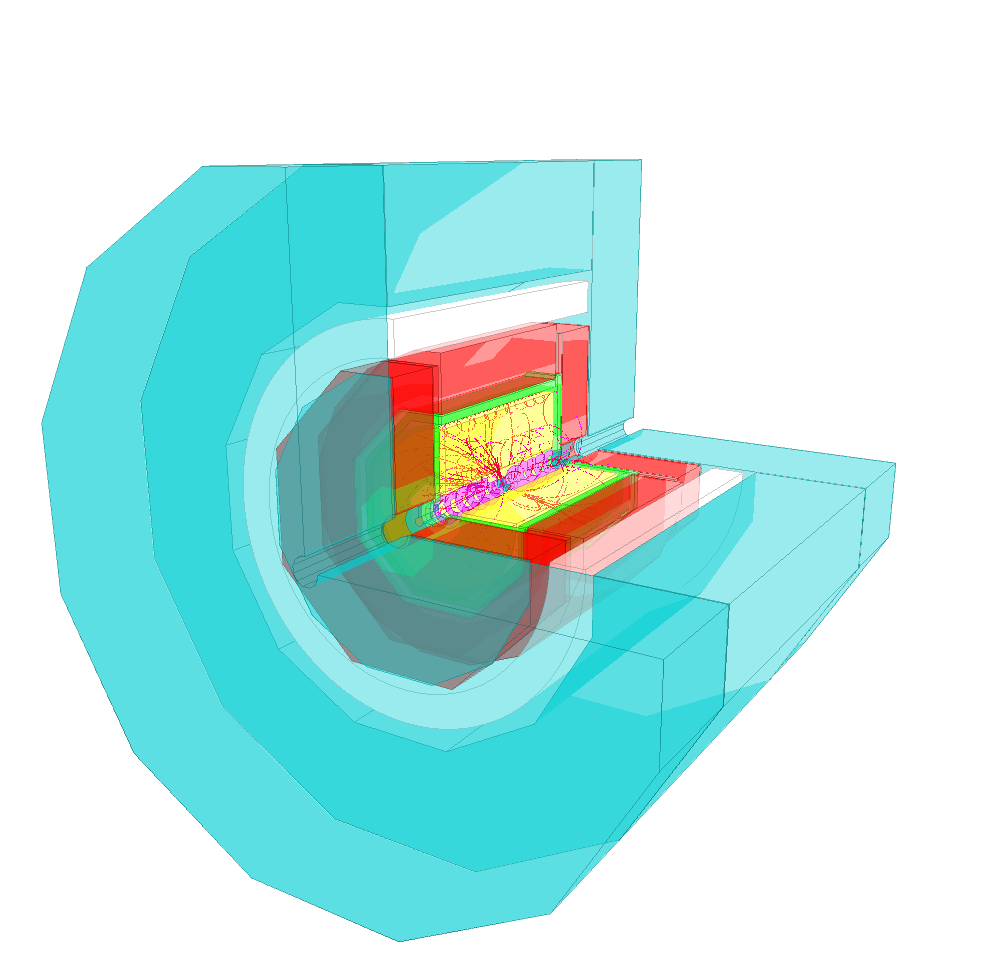
\includegraphics[height=5.5cm]{transparency_60.png}}}
\caption{\label{DSTViewer}\textsl{Transparency 60\%}}
\end{minipage}
\end{figure}

\begin{figure}[h!]
\begin{minipage}[t]{6cm}
\setlength{\fboxsep}{0mm}
\centerline{\fbox{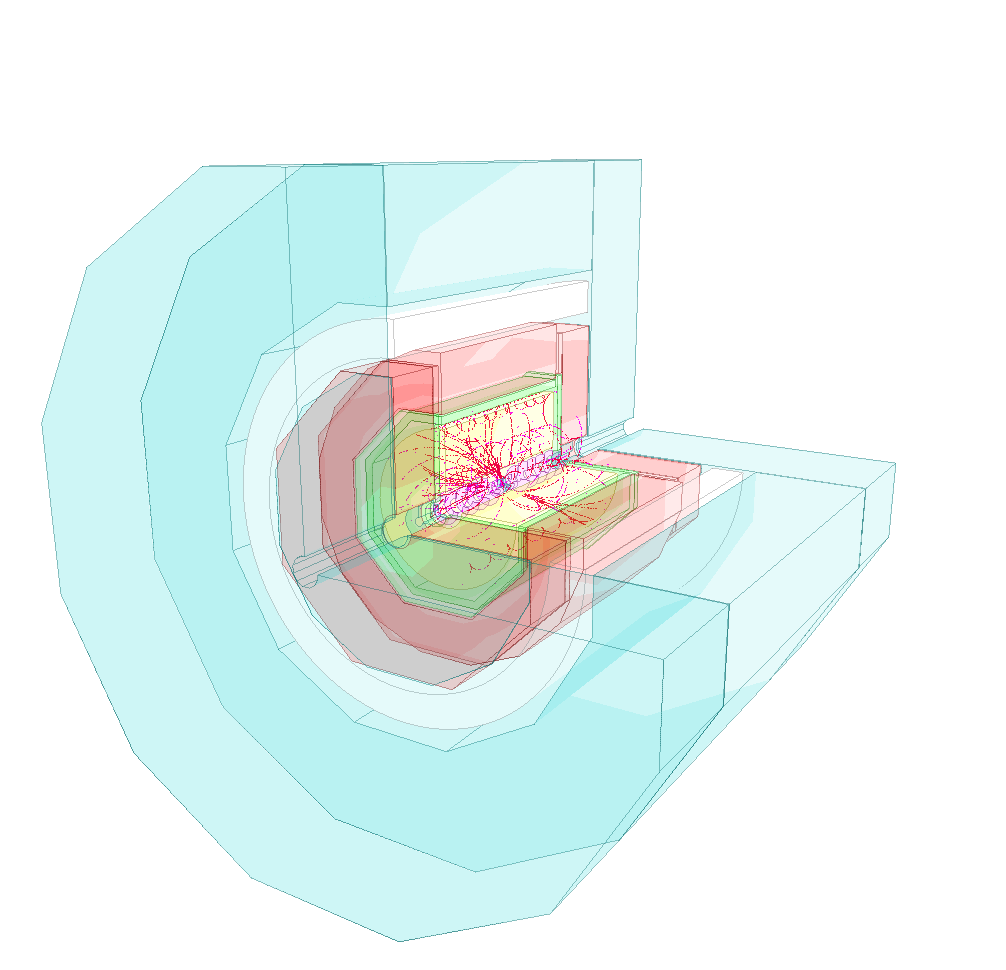
\includegraphics[height=5.5cm]{transparency_90.png}}}
\caption{\label{CEDViewer} \textsl{Transparency 90\%}}
\end{minipage}
\hfill
\begin{minipage}[t]{6cm}
\setlength{\fboxsep}{0mm}
\centerline{\fbox{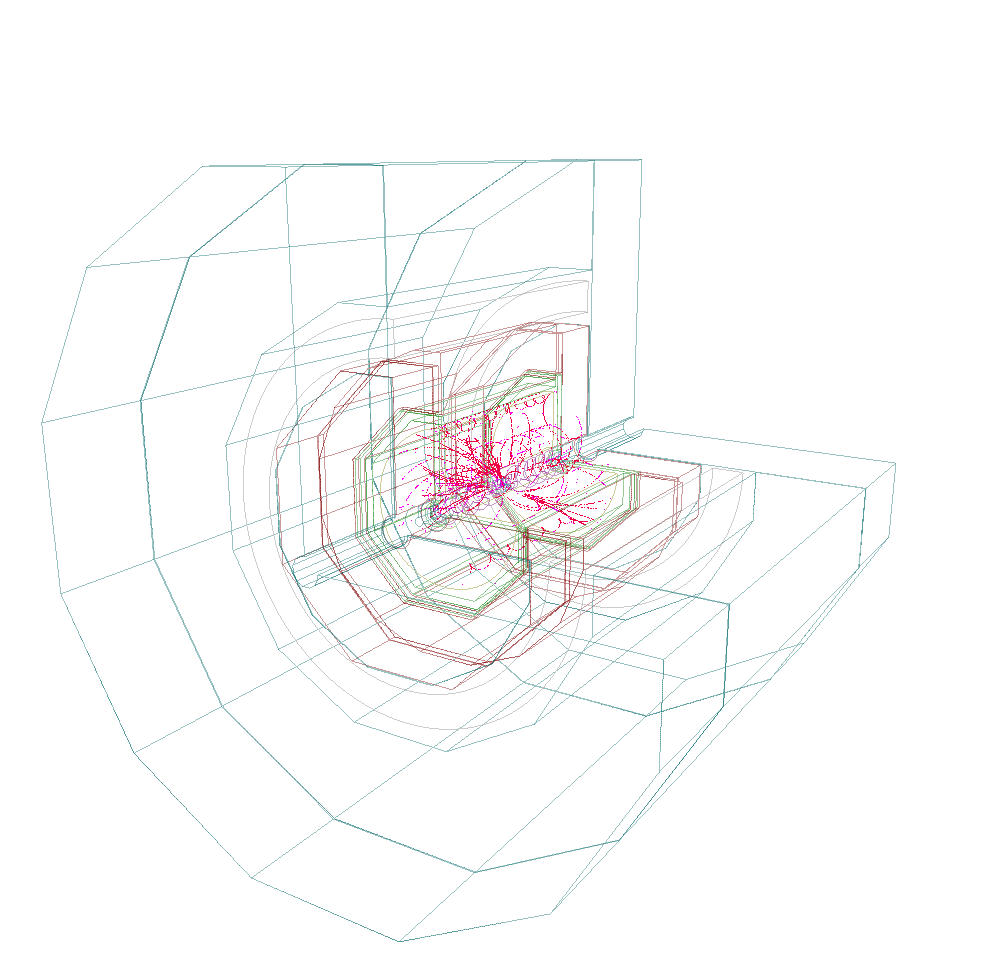
\includegraphics[height=5.5cm]{transparency_100.png}}}
\caption{\label{DSTViewer}\textsl{Transparency 100\%}}
\end{minipage}
\end{figure}

\subsection{Frames per seconds}
To measure the performance of CED, there is a build-in function called 'FPS' (Frames per seconds). Normally CED only renders a new image after changes, such as toggleing the visibility of a layer, or changing the view. In contrast, in FPS mode CED renders so many images as possible and prints out, how many images there were rendered in the last second. This is a good way, to compare the performance of CED in different circumstances, for instance different versions, different viewers, or different machines. 
\newline\newline
Notice: This function is disabled under Mac OSX. 
\section{Picking}
%By selecting a object in CED by double click it, CED send the object ID back to client (usual Marlin).
\subsection{Quickstart}
Simply double click on the object in which you are interested in, Marlin will print out information about the selected object. 
\begin{figure}[h!]
\begin{minipage}[t]{6cm}
\setlength{\fboxsep}{0mm}
\centerline{\fbox{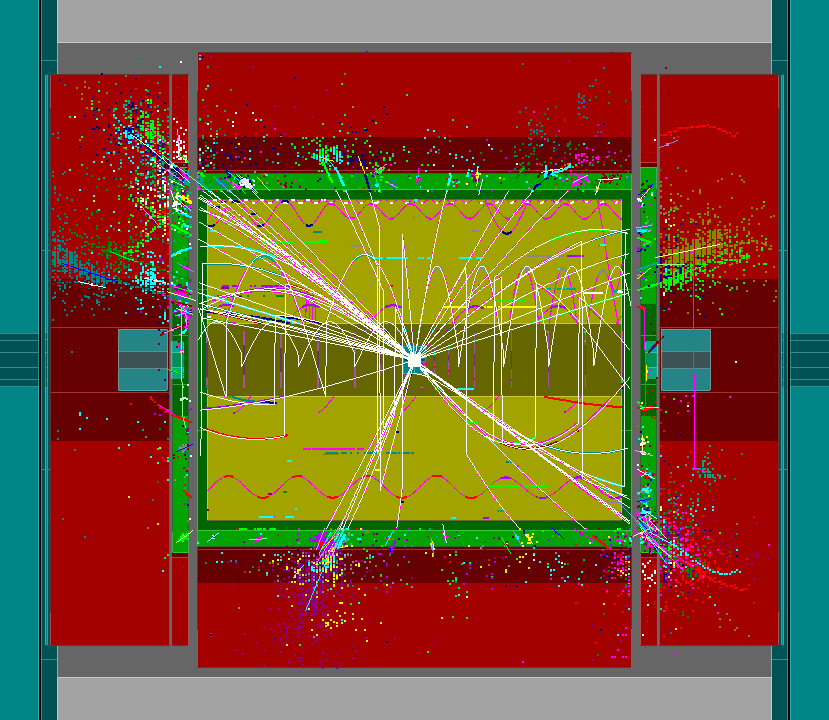
\includegraphics[height=5cm]{picking_ced_window2.png}}}
\caption{\label{CEDViewer} \textsl{CED window}}
\end{minipage}
\hfill
\begin{minipage}[t]{6cm}
\setlength{\fboxsep}{0mm}
\centerline{\fbox{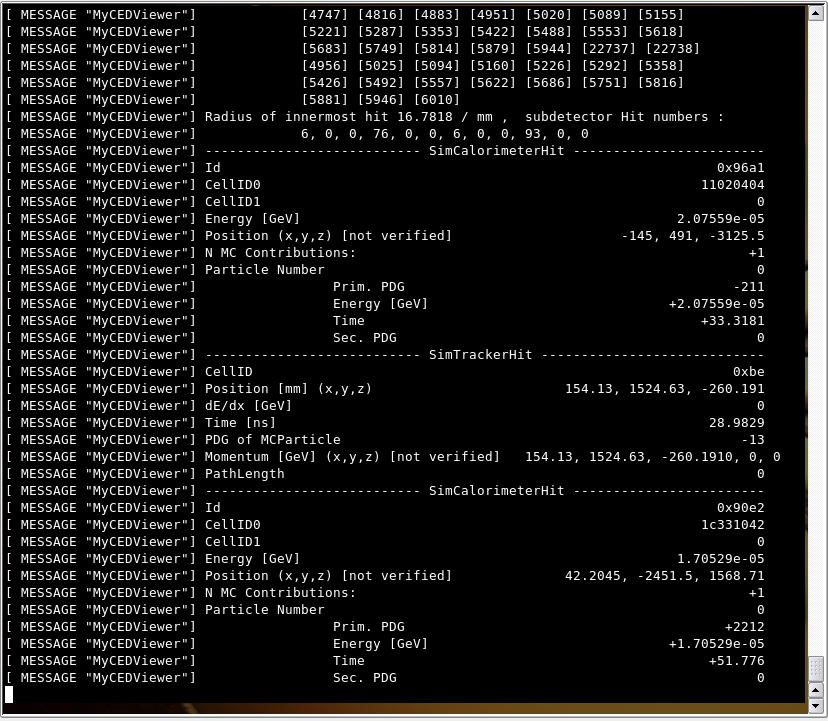
\includegraphics[height=5cm]{picking_terminal_window2.png}}}
\caption{\label{DSTViewer}\textsl{Terminal where Marlin runs}}
\end{minipage}
\end{figure}
 

\subsection{Install your own print function}\label{own_picking}
First, the following code has to be inserted into the processEvent function of the viewer (if you use your own viewer):
\begin{verbatim}
CEDPickingHandler &pHandler=CEDPickingHandler::getInstance();
pHandler.update(evt);
\end{verbatim}

The purpose of this code is, that the singleton class CEDPickingHandler knows all objects of the event and therefore assigns a print function for every object. There are predefined default output functions which can be overwritten by the user. To use your own output functions, it is necessary to register them, before calling the update function. That can be done by
calling the register function. The first argument is a collection name or type and the second argument is a pointer to the print function.
Example:
\begin{verbatim}
CEDPickingHandler &pHandler=CEDPickingHandler::getInstance();
pHandler.registerFunction(LCIO::MCPARTICLE, &MyMCParticlePrintFunction);
//...more printfunctions for other types
pHandler.update(evt);
\end{verbatim}

Note: For a proper use of picking, it is essential that the IDs of every object drawn in CED are communicated to CED. This is done by using the functions ced\_line\_ID instead of ced\_line and ced\_hit\_ID instead of ced\_hit. 
\newline
Within the project, print functions have been designed for a number of LCIO objects. The work of Jan Engels served as a basic principle. This allows to send LCIO objects directly to output streams. It is possible to print LCIO objects in a short or long style. The long form:

\begin{verbatim}
Vertex *vertex = (Vertex *) YourLCIOVertexObjekt;
cout << vertex;
\end{verbatim}
The short form:
\begin{verbatim}
Vertex *vertex = (Vertex *) YourLCIOVertexObjekt;
cout << lc_short(vertex);
\end{verbatim}
The short form allows to print objects as tables:
\begin{verbatim}
Vertex *vertex1 = (Vertex *) YourLCIOVertexObjekt1;
Vertex *vertex2 = (Vertex *) YourLCIOVertexObjekt2;
cout << header(vertex) << tail(vertex) << lcshort(vertex1) << lcshort(vertex2)
<< tail(vertex);
\end{verbatim}
or:
\begin{verbatim}
cout << header(EVENT::Vertex) << tail(EVENT::Vertex) << lcshort(vertex1)
<< lcshort(vertex2) << tail(EVENT::Vertex);
\end{verbatim}
This method of printing is available for the following LCIO types: MCParticle, TrackerHit,
SimTrackerHit, CalorimeterHit, SimCalorimeterHit, ReconstructedParticle, Track and Cluster.

\section{Work with CED from remote}
For a smooth and quick workflow it is always recommended to start CED on the local computer. How to connect which Marlin from a remote computer to your local running CED will be described hereafter.
\newline\newline
To allow incoming remote connections, CED must be started with the option 'trust'. The arguments of this option are a hostname or IP address.
\begin{verbatim}
    #On the local computer
    glced -trust <the name of the remote host>
\end{verbatim}
On the computer on which you will start Marlin, you need to tell Marlin where to connect to by setting the environment variable CED\_HOST.
\begin{verbatim}
    #On the remote computer
    export CED_HOST=<your local hostname>
    Marlin <your datafile>
\end{verbatim}

\section{Change the CED port}
CED binds to a TCP/IP socket to receive data that will be drawn. By default it uses port number 7286. To change it, save the portnumber you want to use in the environment variable CED\_PORT. 
\begin{verbatim}
    export CED_PORT=<Portnumber>
\end{verbatim}
Ensure that the environment variable is set to the same value for Marlin and CED.

\section{CED2go}
This tool is designed to enable a quick and simple view into the events of a data file. To start ced2go type:
 \begin{verbatim}
  ced2go <LCIO File>
 \end{verbatim}
Marlin and CED will be started.
\newline\newline
CED2go will determine which gearfile has been used by generating the LCIO file and configure the viewer(s). If you use your very own gearfile you must tell ced2go where to find it, use the -d \textless Gearfile\textgreater   option. The default viewer is the CEDViewer, use the -v option to change it, more than one viewer at the same time is supported. This information has to be written in a XML file to configure Marlin. Secondly ced2go  search for a free TCP/IP port, so its possible to start ced2go several times. After that, CED will start and Marlin connects.
 
%\subsection{Overview}

%\subsection{ced2go options}
%\section{FAQ}
\section{Viewer}
To draw an event with Marlin into CED, Marlin needs a configuration file, written in XML. This file is called the Marlin-Steeringfile, see its documentation for details. In this file one or more viewers are configured. There a a number of different viewers available in ilcsoft: CEDViewer, DSTViewer, Generic Viewer, and Vertex Viewer. The difference between these viewers is how the event gets drawn. The detector geometry does not depend on with viewer is used. 

A sample viewer configuration section could be:
 \begin{verbatim}
  <execute>
      <processor name="MyGenericViewer"/>
   </execute>

 <processor name="MyGenericViewer" type="GenericViewer">
   <!--Sim Calo Hit Collection Names-->
   <parameter name="SimCaloHitCollections" type="StringVec"
        lcioInType="SimCalorimeterHit"> 
        BeamCalCollection EcalBarrelCollection
        EcalBarrelPreShowerCollection EcalEndcapCollection 
        EcalEndcapPreShowerCollection EcalEndcapRingCollection 
        EcalEndcapRingPreShowerCollection HcalBarrelRegCollection 
        HcalEndCapRingsCollection HcalEndCapsCollection LHcalCollection 
        LumiCalCollection MuonEndCapCollection 
   </parameter>
   
   <!--Sim Tracker Hit Collection Names-->
   <parameter name="SimTrackerHitCollections" type="StringVec" 
        lcioInType="SimTrackerHit"> 
        ETDCollection FTDCollection SETCollection SITCollection 
        TPCCollection TPCSpacePointCollection VXDCollection 
   </parameter>

   <!--Layer for Sim Calo Hits-->
   <parameter name="LayerSimCaloHit" type="int" value="5"/>
   
   <!--Layer for Sim Tracker Hits-->
   <parameter name="LayerSimTrackerHit" type="int" value="6"/>
</processor>

 \end{verbatim}
A viewer is used from Marlin as a library and to specify the style, color and layer of things which get drawn into CED.

Examples of different viewers are shown in Figure \ref{CEDViewer} - \ref{User viewer}. 

\begin{figure}[h]
\begin{minipage}[t]{6cm}
\setlength{\fboxsep}{0mm}
\centerline{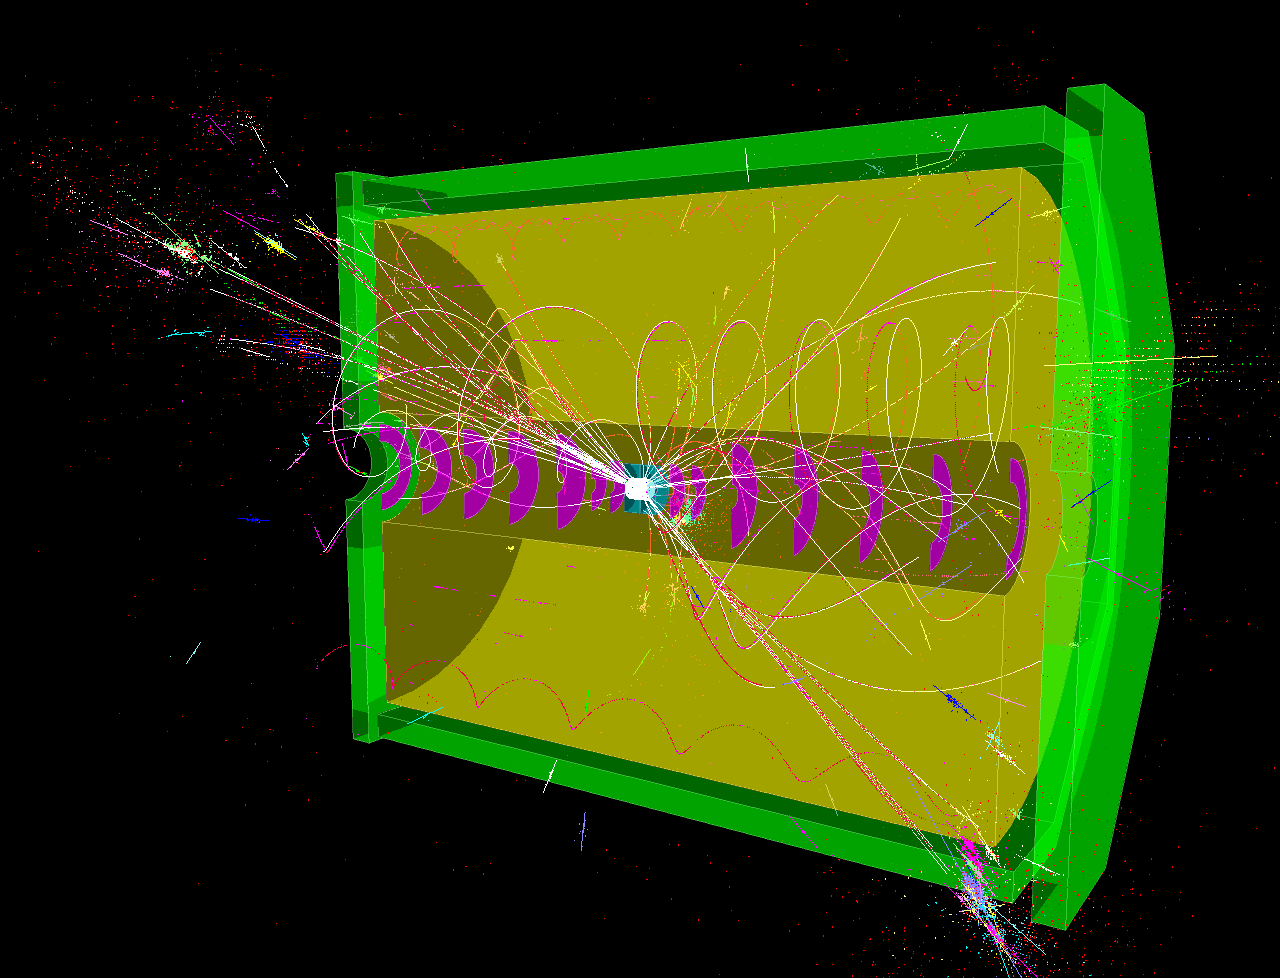
\includegraphics[height=4.4cm]{ced_viewer1.png}}
\caption{\label{CEDViewer} \textsl{CEDViewer}}
\end{minipage}
\hfill
\begin{minipage}[t]{6cm}
\setlength{\fboxsep}{0mm}
\centerline{\fbox{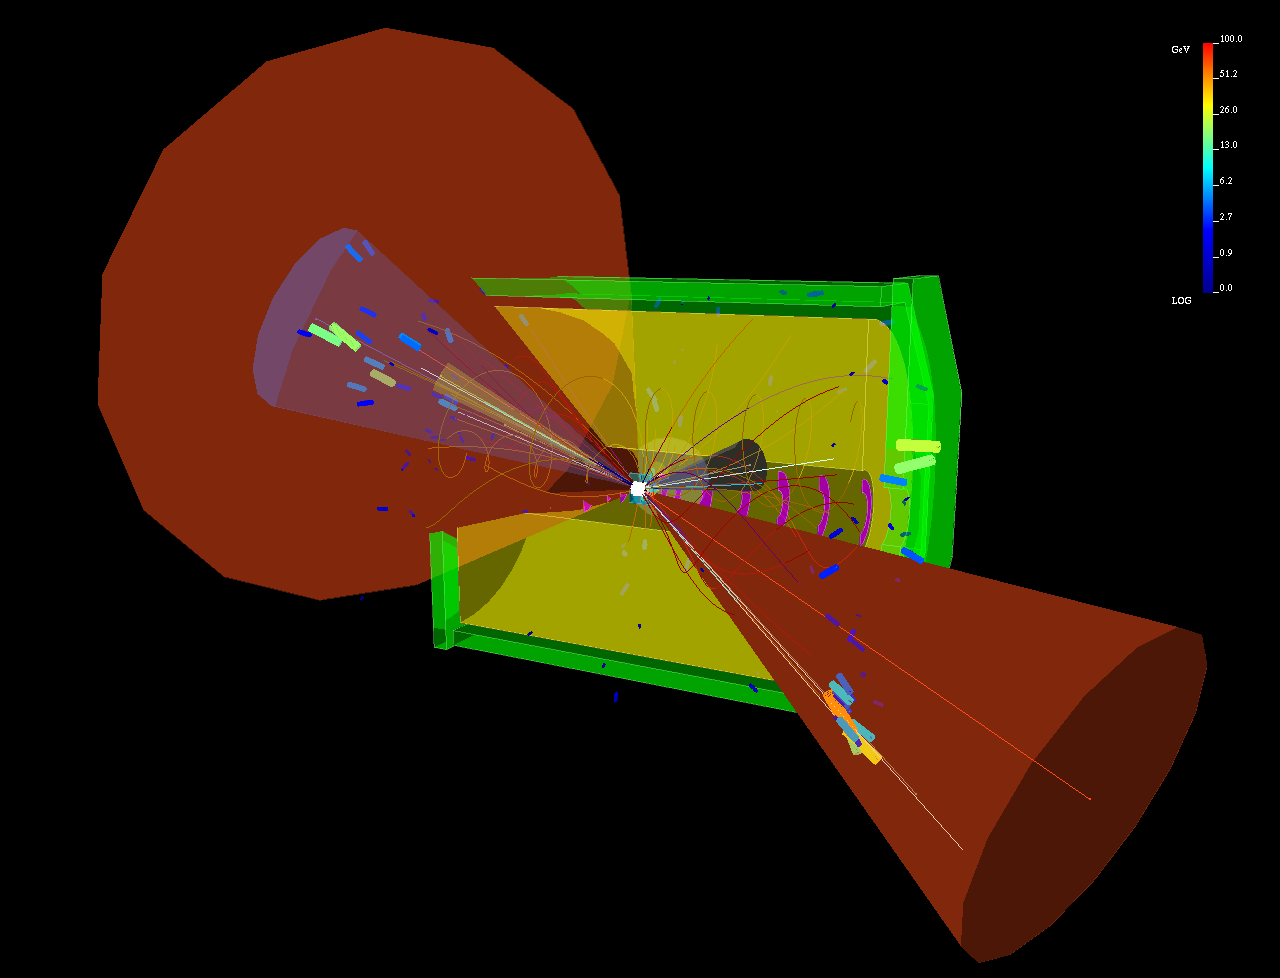
\includegraphics[height=4.4cm]{dst_viewer1.png}}}
\caption{\label{DSTViewer}\textsl{DSTViewer}}
\end{minipage}
\end{figure}

\begin{figure}[h]
\begin{minipage}[t]{6cm}
\setlength{\fboxsep}{0mm}
\centerline{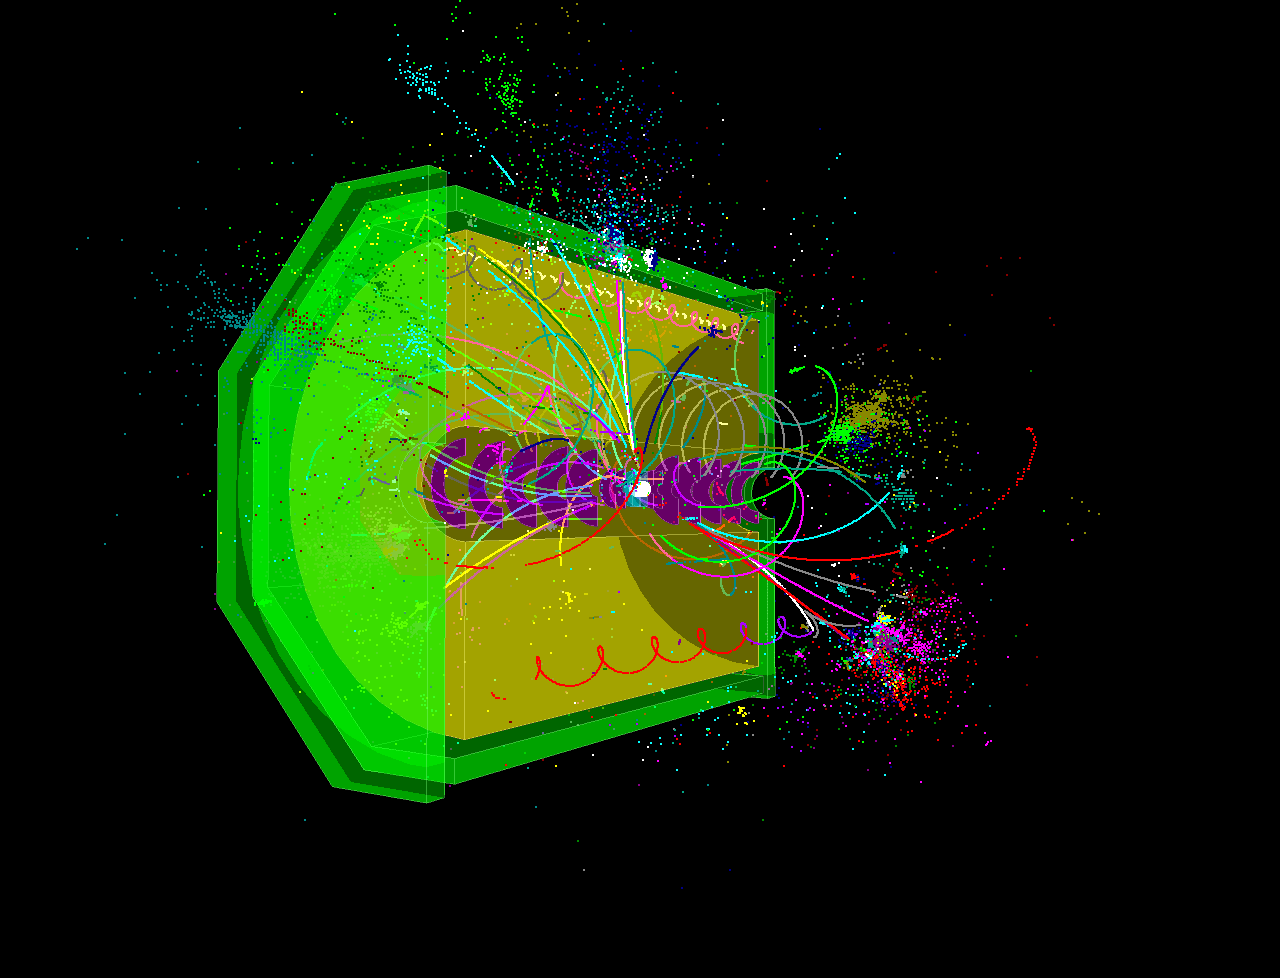
\includegraphics[height=4.4cm]{generic_viewer1.png}}
\caption{\label{GenericViewer} \textsl{GenericViewer}}
\end{minipage}
\hfill
\begin{minipage}[t]{6cm}
\setlength{\fboxsep}{0mm}
\centerline{\fbox{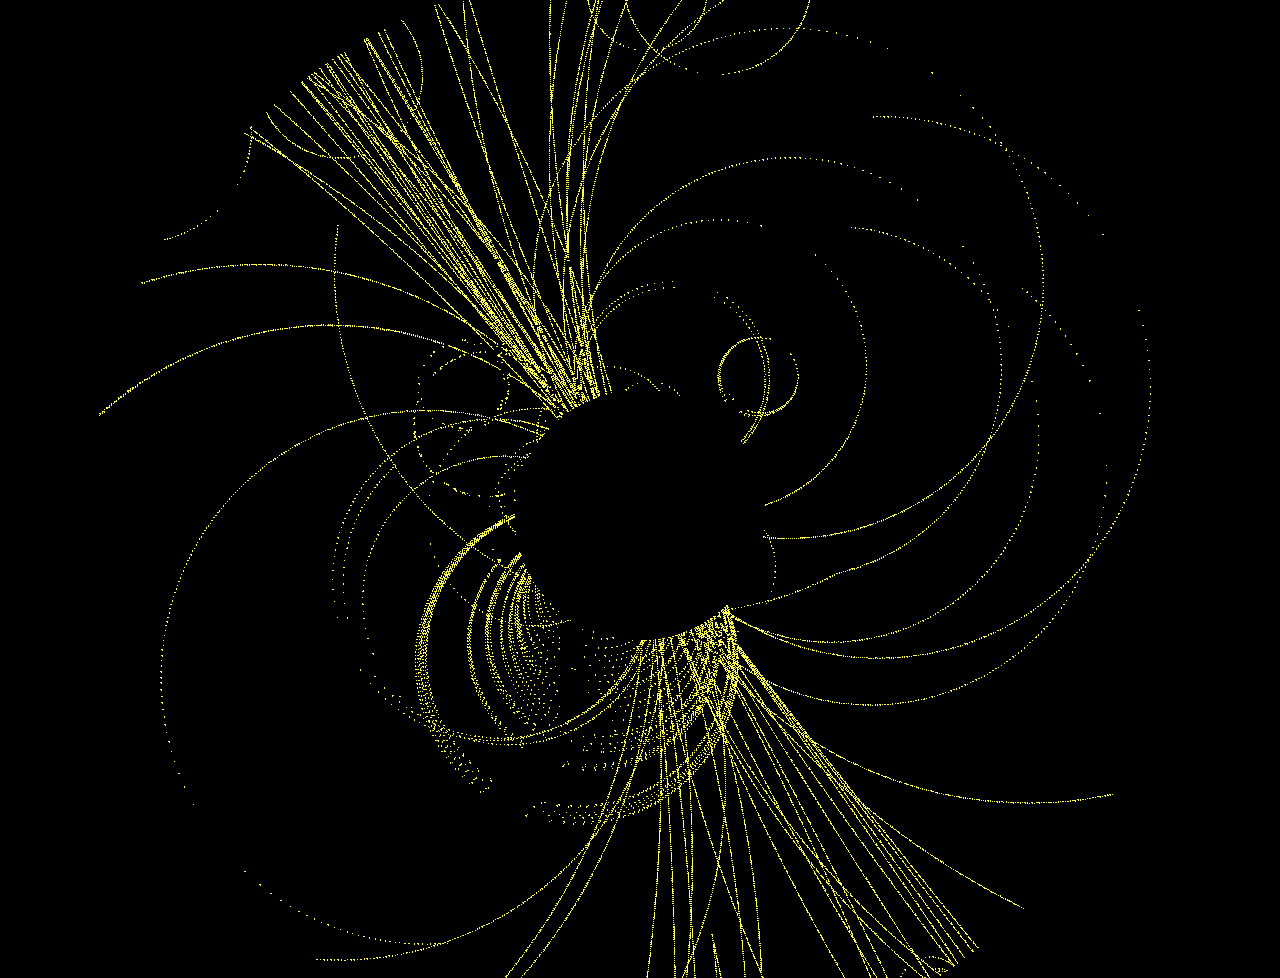
\includegraphics[height=4.4cm]{steve_viewer2.png}}}
\caption{\label{User viewer}\textsl{User defined}}
\end{minipage}
\end{figure}


%\subsection{CEDViewer}

\section{MarlinUtil::MarlinCED}
MarlinUtil::MarlinCED is a library used by Marlin, which provides the functions to draw data into CED. This function simply calls the ced draw functions. It also provides the client part of picking, which means the  mapping between LCIO objects and LCIO ID, and calling the output function of the selected object. For details of the picking part see chapter \ref{own_picking}.

\section{Shortcuts} 
\begin{center}
 \begin{tabular}[ht]{|c|l||c|l|}
  \hline
  Shortcut & Option & Shortcut & Option\\
  \hline\hline
  0 & Toggle layer 0 & b & Toggle background color\\
  1 & Toggle layer 1 & h & Toggle help frame\\
  2 & Toggle layer 2 & r or R & Reset view settings\\
  3 & Toggle layer 3 & f & Front view\\
  4 & Toggle layer 4 & F & Front view projection\\
  5 & Toggle layer 5 & s & Side view\\
  6 & Toggle layer 6 & S & Side view projection\\
  7 & Toggle layer 7 & c or C & Center object at mouseover\\
  8 & Toggle layer 8 & v or V & Toggle fisheye view\\
  9 & Toggle layer 9 & $`$ & Toggle the visible of all data layers\\
  ) & Toggle layer 10 & &\\
  ! & Toggle layer 11 & &\\
  @ & Toggle layer 12 & &\\
  \# & Toggle layer 13 & &\\
  \$ & Toggle layer 14 & &\\
  \% & Toggle layer 15 & &\\
  \textasciicircum  & Toggle layer 16 & &\\
  \& & Toggle layer 17 & &\\
  $\star$ & Toggle layer 18 & &\\
  ( & Toggle layer 19 & &\\
  t & Toggle layer 20 & &\\
  y & Toggle layer 21 & &\\
  u & Toggle layer 22 & &\\
  i & Toggle layer 23 & &\\
  o & Toggle layer 24 & &\\
  \hline
\end{tabular}
\end{center}

\end{document}
